%%%%%%%%%%%%%%%%%%%%%%%%%%%%%%%%%%%%%%%%
%% MCM/ICM LaTeX Template %%
%% 2021 MCM/ICM           %%
%%%%%%%%%%%%%%%%%%%%%%%%%%%%%%%%%%%%%%%%
\documentclass[a4paper,12pt]{article}
\usepackage{geometry}
\geometry{left=0.75in,right=0.75in,top=1in,bottom=0.8in}

%%%%%%%%%%%%%%%%%%%%%%%%%%%%%%%%%%%%%%%%
% Replace ABCDEF in the next line with your chosen problem
% and replace 1111111 with your Team Control Number
\newcommand{\Problem}{A}
\newcommand{\Team}{2106187}
%%%%%%%%%%%%%%%%%%%%%%%%%%%%%%%%%%%%%%%%

\usepackage{newtxtext}
\usepackage{amsmath,amssymb,amsthm}
\usepackage{newtxmath} % must come after amsXXX
 \setlength{\itemsep}{0ex} %条目间距
  \setlength{\topsep}{5ex} %列表到上下文的垂直距离
\usepackage{palatino}
\usepackage{booktabs}
\usepackage{mwe}
\usepackage{subcaption}
\usepackage{float}
\usepackage{multirow}
\usepackage{indentfirst}
\usepackage{gensymb}
\usepackage[ruled,lined,commentsnumbered]{algorithm2e}
\usepackage{diagbox}

%\usepackage[pdftex]{graphicx}
\usepackage{xcolor}
\usepackage{fancyhdr}
\lhead{Team \Team}
\rhead{page \thepage of \pageref{LastPage}}
\cfoot{}
\usepackage[utf8]{inputenc}
\usepackage[T1]{fontenc}
\usepackage{textcomp}
\usepackage{listings}
% 在LaTex中添加代码
\usepackage{color}
\usepackage{lastpage}
\usepackage{graphics,pdfpages}

\definecolor{codegreen}{rgb}{0,0.6,0}
\definecolor{codegray}{rgb}{0.5,0.5,0.5}
\definecolor{codepurple}{rgb}{0.58,0,0.82}
\definecolor{backcolour}{rgb}{0.95,0.95,0.92}
 
\lstdefinestyle{mystyle}{
    backgroundcolor=\color{backcolour},   
    commentstyle=\color{codegreen},
    keywordstyle=\color{magenta},
    numberstyle=\tiny\color{codegray},
    stringstyle=\color{codepurple},
    basicstyle=\footnotesize,
    breakatwhitespace=false,         
    breaklines=true,                 
    captionpos=b,                    
    keepspaces=true,                 
    numbers=left,                    
    numbersep=5pt,                  
    showspaces=false,                
    showstringspaces=false,
    showtabs=false,                  
    tabsize=2
}
\lstset{breaklines=true}
\usepackage[framed,numbered]{mcode}

\newtheorem{theorem}{Theorem}
\newtheorem{corollary}[theorem]{Corollary}
\newtheorem{lemma}[theorem]{Lemma}
\newtheorem{definition}{Definition}
\renewcommand{\abstractname}{\large Summary \\}
%\renewcommand{\contentsname}{}

%%%%%%%%%%%%%%%%%%%%%%%%%%%%%%%%
\begin{document}
\graphicspath{{.}}  % Place your graphic files in the same directory as your main document
\DeclareGraphicsExtensions{.pdf, .jpg, .tif, .png}
\thispagestyle{empty}
\vspace*{-16ex}
\centerline{\begin{tabular}{*3{c}}
	\parbox[t]{0.3\linewidth}{\begin{center}\textbf{Problem Chosen}\\ \Large \textcolor{red}{\Problem}\end{center}}
	& \parbox[t]{0.3\linewidth}{\begin{center}\textbf{2021\\ MCM/ICM\\ Summary Sheet}\end{center}}
	& \parbox[t]{0.3\linewidth}{\begin{center}\textbf{Team Control Number}\\ \Large \textcolor{red}{\Team}\end{center}}	\\
	\hline
\end{tabular}}
%%%%%%%%%%% Begin Summary %%%%%%%%%%%
% Enter your summary here replacing the (red) text
% Replace the text from here ...



\begin{center}

\textbf{Optimization of the future transportation:\\ Lightweight Suspension Transportation System
\bigskip
\\Summary} 
\end{center}



\bigskip

Key words: Fungi, Elo system, CA modeling, Species Interaction \& Competition, Climate, Diversity
% to here
%%%%%%%%%%% End Summary %%%%%%%%%%%

%%%%%%%%%%%%%%%%%%%%%%%%%%%%%%
\clearpage
\pagestyle{fancy}
% Uncomment the next line to generate a Table of Contents
%\tableofcontents 
\newpage
\setcounter{page}{1}
\rhead{Page \thepage\ of \pageref{LastPage}}
%%%%%%%%%%%%%%%%%%%%%%%%%%%%%%
\tableofcontents


\newpage


\section{Introduction}

\subsection{Background}

\par The carbon circle plays an important role in the operation of ecosystem on Earth. While plants transform the inorganic carbon in the environment into organics, there must be some other creatures transforming organics back. As the primary decomposers of ground litter and woody fibers in ecosystems, fungi are critical agents of the global carbon cycle \cite{CompArticle}. According to an article of a recent research, there are some fungi traits influencing the decomposition rate, including the growth rate (described by the hyphal extension rate), and the moisture tolerance \cite{CompArticle}. The traits vary between different species of fungi, and the research shows: those fungi with higher growth rate and competitiveness decompose materials faster; while the fungi which grow slower, with better adaptation to different moisture conditions, decompose the materials slower \cite{CompArticle}. 

\begin{figure}[H]
	\centering
	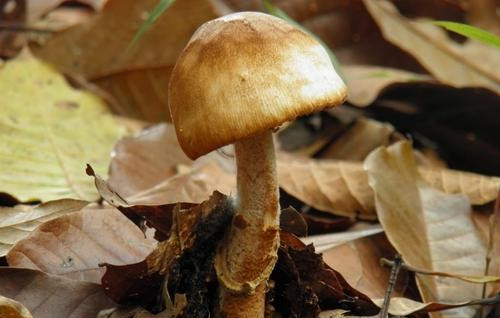
\includegraphics[width=0.4\textwidth]{./figures/fungi.jpeg}
	\caption{A mushroom (a type of fungi) decomposing the dead plant material \cite{mushroom}.}
	\label{mushroom}
\end{figure}

\subsection{Analysis \& Problem Restatement}

\par In this problem, we need build models to describe the decomposition process of ground litter and woody fibers in a certain area, with multiple species of fungi existing. Apart from the two traits of fungi, we also need to take the interaction of fungi species into consideration. When the environmental factors change, the growth rate of fungi, the interaction between species, as well as the decomposition rate will change. Hence, for this problem, the work to do includes:

\begin{enumerate}
 \setlength{\itemsep}{0ex} %条目间距
\item For a certain amount of ground litter and woody fibers, build a mathematical model to relate the decomposition process with the traits (different growth rates and moisture tolerances) of different species of fungi there. Take the interaction of those multiple fungi species into account.
\item How do different species of fungi interact with each other? Analyze the trends of interactions in both the short-term case and the long-term case. In the analysis, the impacts of following environmental factors should be included: rapid fluctuations (sensitivity analysis), changes of atmosphere trends (local whether pattens).
\item For five different environments (arid, semi-arid, temperate, arboreal, and tropical rain forests), analyze the relative advantages and disadvantages of different species of fungi, and predict which kinds of species combinations tend to exist persistently. 
\item By considering the breakdown rate of ground litter, describe the impact of diversity of fungi on the efficiency of ecosystems. Predict the effect and significance of biodiversity on the diversity of local environments.
\end{enumerate}

\section{Model Preparation}
\subsection{Assumptions}
In order to simplify the problem and extract an effective model for solving it, the following assumptions are made: 
\begin{enumerate} 
\setlength{\itemsep}{0ex} %条目间距
\item The decomposition rate is only influenced by two traits of the fungi: the \textbf{hyphal extension rate} and the \textbf{moisture tolerance}. Although other traits may also influence the decomposition rate, they are not the focus of this problem.
\item \textbf{The only decomposer} in this problem is the fungi. Other creatures (such as bacteria) will make \textbf{no} contribution to the decomposition processes.
\item We only consider the growth (namely the hyphal extension) of fungi, and \textbf{reproduction is excluded from the problem}. Besides, each unit piece of hyphal of the same fungus will decompose the material \textbf{at a constant rate} over time, as long as the environmental conditions do not change, until all the material it covers is decomposed.  
\item The decomposition rates do \textbf{not} vary between different types of ground litter and woody fibers. In other words, all the material to be decomposed are \textbf{homogeneous}.
\item \textbf{The only environmental factors} influencing the decomposition rate of material is \textbf{moisture}. Any other environmental factors, such as winds, sunshine, the acidity of soil, and the existence of certain chemicals, are \textbf{not} taken into consideration.
\end{enumerate}

\subsection{Notations}
For clarity, the notations used for the models are listed in Table \ref{notation}. \textbf{(Note: The $^*$ marked on the definitions indicates that the symbols represent quantities of a single species of fungus. Those quantities varies between different fungi species.)}
\begin{table}[H]
	\centering
	\caption{Notations}
	\begin{tabular}{lll}
	\midrule
	Symbol & Definition & Unit\\
	\hline
	$D$ & Decomposition Rate$^*$ & \% (of mass)/122 day \\
	$D_{1}$ & The part of $D$ determined by hyphal extension rate$^*$ & \% (of mass)/122 day\\
	$D_{2}$ & The part of $D$ determined by moisture tolerance$^*$ & \% (of mass)/122 day\\
	$\omega$ & The weight of $D_1$ in $D$ & \\
	$E$ & Hyphal extension rate$^*$ & mm/day \\
	$E_{0}$ & Maximum extension rate at the optimal moisture$^*$ & mm/day\\ 
	$M_{t}$ & Moisture trade-off/ moisture tolerance$^*$ &  \\ 
	$m_{0}$ & The optimal moisture$^*$ & Mpa \\
	$m$ & Moisture at the moment$^*$ & Mpa \\
	$R$ & Competitiveness ranking of a fungus species$^*$ & \\ 
	$B$ & Moisture niche width (scaled to $[0,1]$)$^*$ & \\ 
	$L$ & Total length of the hypha$^*$ & mm\\ 
	$l_0$ & Initial length of the hypha$^*$ & mm \\ 
	$t$ & Elapsed time (from the beginning of decomposition) & day\\
	$x$ & Mass of material decomposed in one day$^*$ & g/(mm $\cdot$ day) \\
	$W_0$ & Original mass of materials in a cell & g \\
	$W$ & Mass of materials in a cell after consuming & g \\
	\bottomrule
	\end{tabular}
	\label{notation}
   \end{table}



\section{Model of Wood Breakdown by Multiple Fungi Species}

\subsection{Model Overview}
\par In order to simulate the real process of fungi's growth, consumption  and competition, CA modeling is used to create a dynamic evolutionary process, making it more convenient to analyze. To drive the whole process, the model is divided into three parts: 
\begin{enumerate}
\setlength{\itemsep}{0ex} %条目间距
\setlength{\topsep}{.1ex} %列表到上下文的垂直距离
	\item Define and calculation the decomposition rate w.r.t. extension rate as well as moisture tolerance. Considering also the effect moisture have on the extension rate
	\item Define the situation and solution when two fungus meet and compete using the competitive ranking. Elo system is adapted which has been proved to be quite efficient.
	\item Apply CA modeling to explicitly show the process of the wood occupation and interactions between fungi.
\end{enumerate}
\par Then, various kind of figures are used to demonstrate the result: 2D maping used for showing the process of fungi growth, line chart for showing the variation of area occupation of multiple fungi and surface plots used for reflecting the number of hypha as well as the consumption of materials.

\subsection{Calculating Decomposition Rate}
The decomposition rate is related with both the extension rate (growth rate) and moisture tolerance. The extension rate can be affected by the species of fungi, its moisture niche range and the exact environment moisture. Thus it can be obtained by Eqn. \ref{E}.
\begin{equation}\label{E}
E=\left\{ \begin{array}{c}
E_0 \qquad \qquad \qquad \qquad  \qquad \qquad  \text{when m} \in  [m_{min},m_{max}] \\
E_0 \times e^{- min\{|m-m_{min}|,|m-m_{max}|\} } \qquad \text{when m} \notin  [m_{min},m_{max}] 
\end{array} \right.
\end{equation}
The tolerance of moisture is defined to be the difference between the fungi isolate's competitive ranking and moisture niche width, both scaled to [0,1]. 
\begin{align*}
M_t=R-B 
\end{align*}
Since the ranking data obtained from the article is already scaled among 34 different species \cite{CompArticle}, we modify each ranking by Eqn. \ref{ranking} when the chosen species for the model is much smaller.
\begin{equation}\label{ranking}
R^{'}_i= \dfrac{R_i}{\sqrt{\sum_{i=1}^n R_i^2}}
\end{equation} where $R_i$ denotes the $i^{th}$ isolate among the n selected species.

The relation between both factors and the decomposition rate can be obtained from a research article by Lustenhouwer, et al\cite{CompArticle} which is shown as the equation below.
\begin{align*}
\left\{ \begin{array}{c}
log(D)=0.32 log(E)+12.48 \\
log(D)=0.82M_t+1.87
\end{array} \right.  \quad \rightarrow \quad  \left\{ 
\begin{array}{c}
D_1(E)= 12.48 \times E^{0.32}\\
D_2(M_t)= e^{0.82M_t+1.87}
\end{array} \right.
\end{align*} 
Since above are the only two traits that is considered in affecting decomposition rate, thus we combine the two relationship using a weight constant:
\begin{equation}\label{weight}
D=\omega \times D_1 + (1-\omega) \times D_2
\end{equation}
However, since the unit for extension rate is mm/day while the calculation for decomposition rate is the percentage mass loss over 122 days. Thus to simplify model calculation, we further derived the equation for calculating the mass consumption per day per unit length of one certain fungus. Using Eqn. \ref{weight}, we then solve for x to get the assumption rate which is described as grams of wood per day, also considering the length growth of the fungi w.r.t. time.
\begin{align*}
L&=l_0 + Et \\
D&=\int_0^{122} Lx dt=\omega \times D_1 + (1-\omega) \times D_2
\end{align*}


\subsection{Competition and Ranking}
From Lustenhouwer's work, the condition for single fungus isolate consuming wood is already clear. However, the model need to describe and predict the decomposition and living condition when multiple fungus species are present. Thus we need to determine a rule for competition between different species when they meet each other.The  moisture tolerance includes an interesting factor called competitive ranking, which is exactly what we need.

The competitive ranking reflects the ability for a fungus to out-compete other fungi in pair-wise testing under the same condition \cite{MCM}. The ranking is tested in reality and calculated following the Elo ranking system which is commonly used among chess players. According to the Elo ranking system, the score is calculated based on all previous competition results and can be used to predict future odds of players \cite{chess}. Also, each competition affects the involved players. The prediction and the modification of ranking formula can also be directly applied to the eco-system with a simple change of parameter K.
\begin{align*}
\left\{ \begin{array}{c}
E_A= \dfrac{1}{1+10^{(R_B-R_A)/k}} \\
E_B= \dfrac{1}{1+10^{(R_A-R_B)/k}}
\end{array} \right. \qquad  \left\{ \begin{array}{c}
R^{'}_A=R_A + K(S_A-E_A) \\
R^{'}_B=R_B + K(S_B-E_B)
\end{array} \right.
\end{align*} where $E_A$ and $E_B$ reflects the possibility of each play to win, while $R_A$ and $R_B$ denotes their competitive ranking. k is the constant found especially for the fungi eco-system. $R^{'}_A$ and $R^{'}_B$ are the modified ranking after each competition.

\subsection{Predicting the Breakdown Process Using CA Modeling}
In order to demonstrate the growth and competition among multiple fungi species, we adapt the cellular automata modeling as the main model structure. Cellular automata is a model that defines \textbf{a finite space} and a series of \textbf{discrete cells}. These cells will automatically evolve according to the different states of their eight \textbf{neighbors} and follow certain \textbf{evolution rules}. It is a dynamic and discrete system which can simulate the growth, decomposition and competition of various fungi on the wood very well. Fig.(\ref{f1ForCA}) shows a brief sketch of cellular automata model.


\par Fig.(\ref{AS}) is the \textbf{evolution rules} for the fungi cell. In the whole process, the growth speed of the cell follows the modified extension rate which is shown on Eqn.\eqref{???}, the winning probability is defined by Elo rating system which is shown on Eqn.\eqref{???} and the decomposition rate is calculated by Eqn.\eqref{???}.

\begin{figure}[] 
	\centering 
	\begin{minipage}{40ex}
	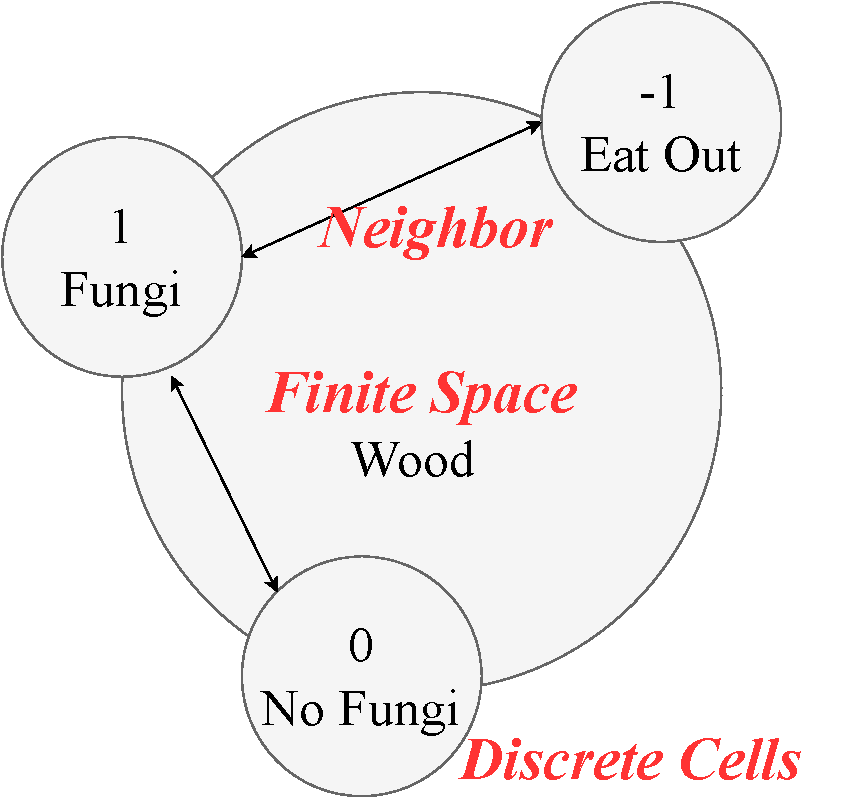
\includegraphics[height=6cm]{./picture/CA.pdf}
	\caption{Cellular automata model}
	\label{f1ForCA}
	\end{minipage}
	\begin{minipage}{40ex}
	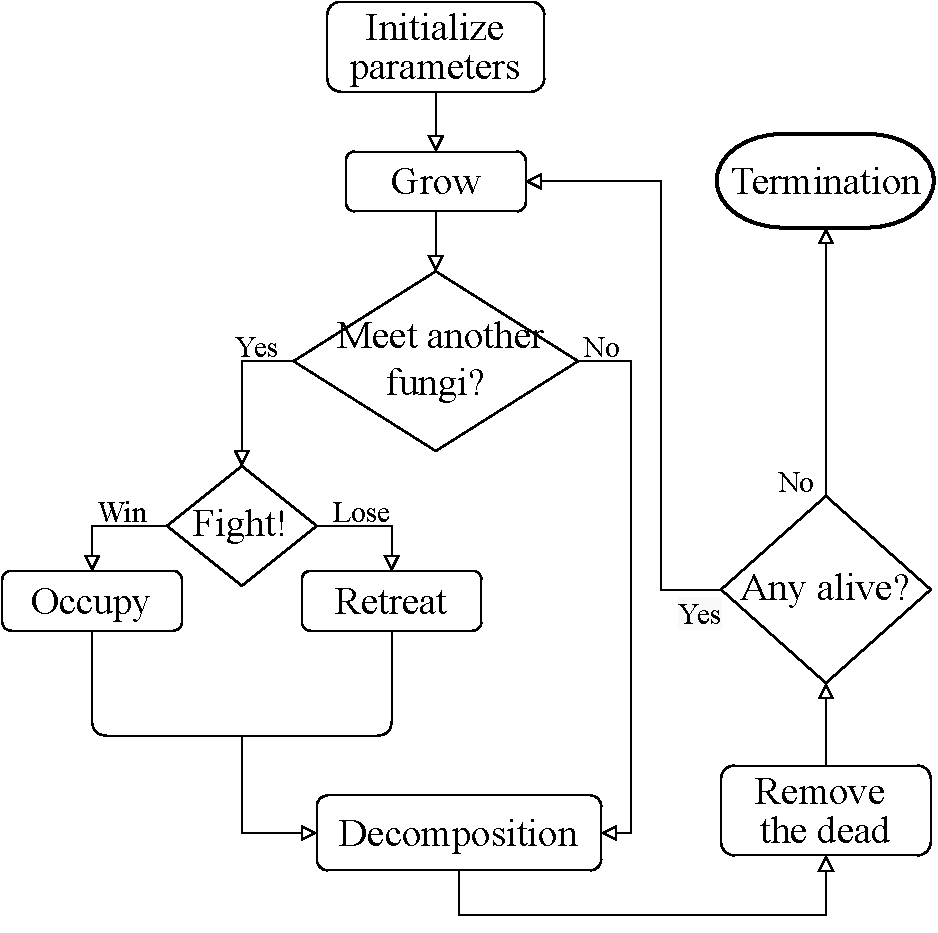
\includegraphics[height=6cm]{./picture/liucheng.pdf}
	\caption{Algorithm schematic.}
	\label{AS}
	\end{minipage}
\end{figure}

Since the data for extension rate we obtained is corrected to two decimal places, we define a wood plate with the same area of the CA model as the land for growing fungi, and assume that the wood is abundant enough during the time period of the whole prediction process (which means the wood won't be completely consumed). Thus we define the size of our CA model to be a \textbf{300 $\times$ 300 map} with each cell having a side length of 0.01 mm for the demonstrations. 

For each single cell, there're properties include the original mass of materials W per cell, the total length of fungus in a single cell, the current remaining mass of materials and the name of the fungus occupying it.  According to CA modeling, the condition of each cell may be affected by adjacent cells. Thus, the growth of the fungus is defined to be extending both vertically and horizontally. Each time when the fungi occupied a new cell, it'll start growing from the new cell as well on the next day. An explicit demonstration is shown in Fig. \ref{wood} where we assume the fungi grow 0.01 mm longer each day.

When two different fungi meet each other during their growth, competition occur to judge which one takes up the cell. Since the extension rate of different fungi are not the same, we assume competition only happens at the cell when the two fungi meet and won't affect those cells that haven't been occupied. Fig. \ref{compete} demonstrates the condition. It's clear that once two fungi start competing, the competition won't end immediately since adjacent cells are always occupied by either fungus.

\begin{figure}[H] 
\captionsetup{font={small}}
	\begin{minipage}{45ex}
	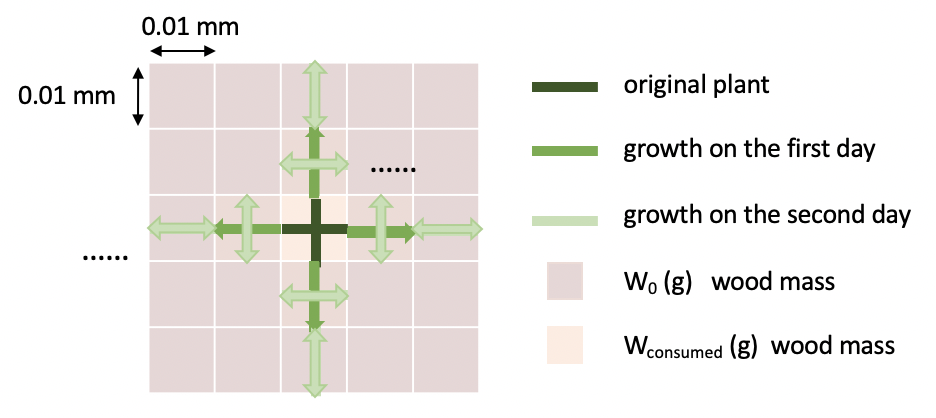
\includegraphics[height=4.3cm]{./figures/wood}
	\caption{Demonstration of the growth modeling (assume the fungi grow 0.01mm longer each day).}
	\label{wood}
	\end{minipage} \quad
	\begin{minipage}{45ex}
	\qquad \quad
	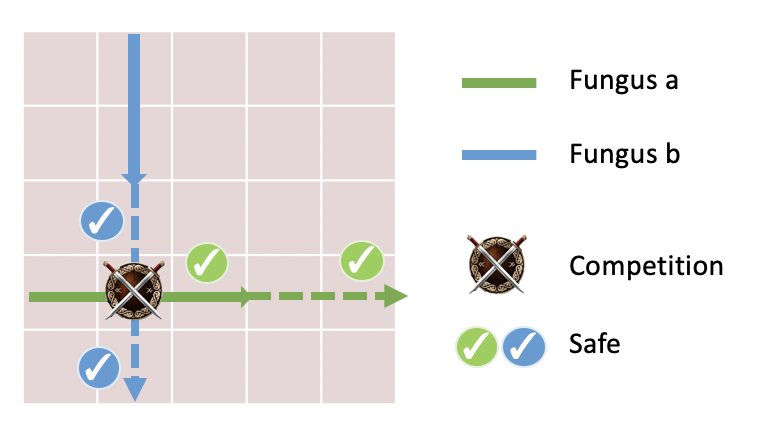
\includegraphics[height=4.2cm]{./figures/compete}
	\caption{Demonstration of the competition (one fungus grow into a cell taken up by the other).}
	\label{compete}
	\end{minipage}
\end{figure}


Finally, since the materials are limited, and we first take the material's reproduction out of consideration. Thus, when the fungus consumed all materials in a certain cell, the cell is changed to death and all the fungus living currently in this cell also die immediately. Once a cell is dead, no more fungus can ever come in and occupy it no matter how it grows. 

\subsection{The Effect of Hypha Thickness in Interactions}
\par Based on the work above, we are now going to make an improvement on the model of interactions between fungi. In the above parts, results of competitions are only influenced by rankings and extension rates of fungi. Therefore, if the ranking of a fungus (called fungus A) is much higher than the other one (fungus B), it will be very likely to occupy nearly all the area that fungus B owns. However, there should be a balance in the real case. Consider that the fungus B starts growing at a point (called the initial point). As time goes on, there should be more hyphae around the initial point of fungus B than at the edge of extension of fungus A. In other words, hyphae on the area around initial point of growing are thicker, thus more difficult to be replaced by other species. As a result, uncompetitive fungi tend to grow persistently in a small area, even though they are surrounded by competitive fungi.
\begin{align*}
	\label{lambda}
	\lambda &=\frac{2}{1+3e^{-\ln3 y}} \quad (y>0)\\
	y &=f(d,\frac{R_A}{R_B})=
	\begin{cases}
		e^{-k_1d} & \frac{R_A}{R_B}>1\\
		\ln (k_2d+e)&\frac{R_A}{R_B}<1\\
	\end{cases}
\end{align*}
\par As shown in the above equations, we introduce two new quantities $d$ and $\lambda$. $d$ is the hyphal thickness of the fungus B (the fungus being attacked), and $\lambda$ is the winning coefficient, in the form of a Logistic function. The larger $\lambda$ is, the higher probability that fungus A will take over the cell. $R_A$ and $R_B$ are the rankings of fungi A and B, respectively. In this example, $\frac{R_A}{R_B}$ is greater than 1. If $\frac{R_A}{R_B}$ is smaller than 1, namely fungus B is more competitive than A, the equations can still be applied. For the case of $R_A=R_B$, we quantify the effect of $d$ by $\Delta(d)$, as shown in Eqn.~\eqref{Delta_d}. With $\lambda$ and $\Delta$, The expressions of fungi A's and B's opportunities to win are modified into Eqn.~\eqref{modified}.
\begin{eqnarray} \label{Delta_d}
	\Delta(d)=
	\begin{cases}
		k_3 \ln (\frac{x}{l_0}+1) & R_A=R_B\\ 
		0 & R_A \neq R_B\\
	\end{cases}
\end{eqnarray}
\begin{equation}
	\label{modified}
	E_A=\frac{1}{1+10^{\lambda(R_B-R_A)}}-\Delta(d), \quad E_B=\frac{1}{1+10^{\lambda(R_A-R_B)}}+\Delta(d)  
\end{equation}

\section{Visualization}
In order to demonstration the process of fungi growth as well as their properties including occupied area, fungi total length and their consumption of wood materials, we made the following visualization including mapping, line charts and surface plotting. Fig. \ref{Eg_colony200} to Fig. \ref{Eg_colony1500} shows their movement and extension, while Fig \ref{Eg_area} to Fig. \ref{Eg_wood} reflects the three properties just mentioned.

\begin{figure}[H]
	\centering
	\begin{subfigure}{0.3\textwidth}
		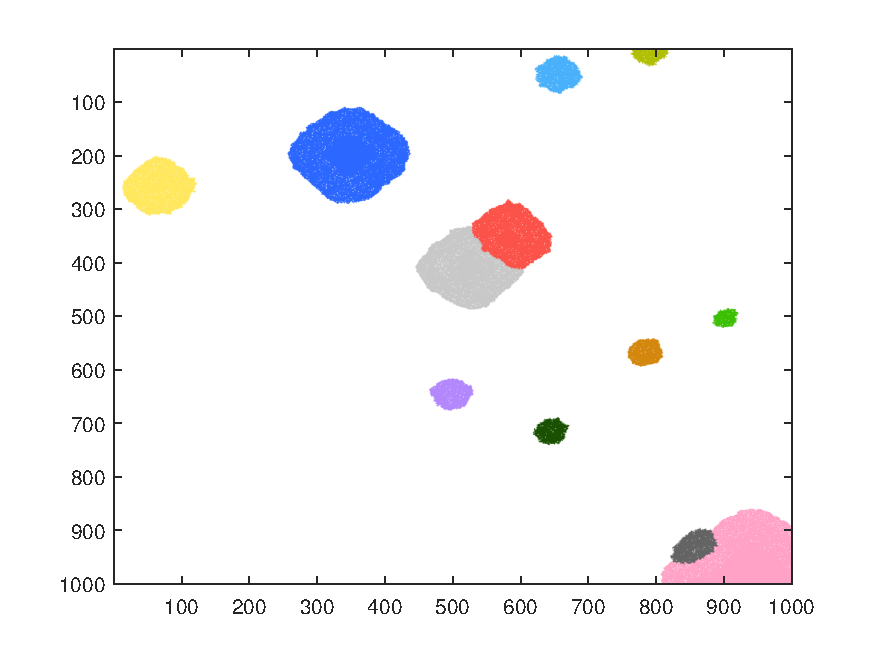
\includegraphics[width=\textwidth]{./picture/Eg_200day.pdf}
		\caption{Colony at t = 200 days}
		\label{Eg_colony200}
	\end{subfigure}
	\begin{subfigure}{0.3\textwidth}
		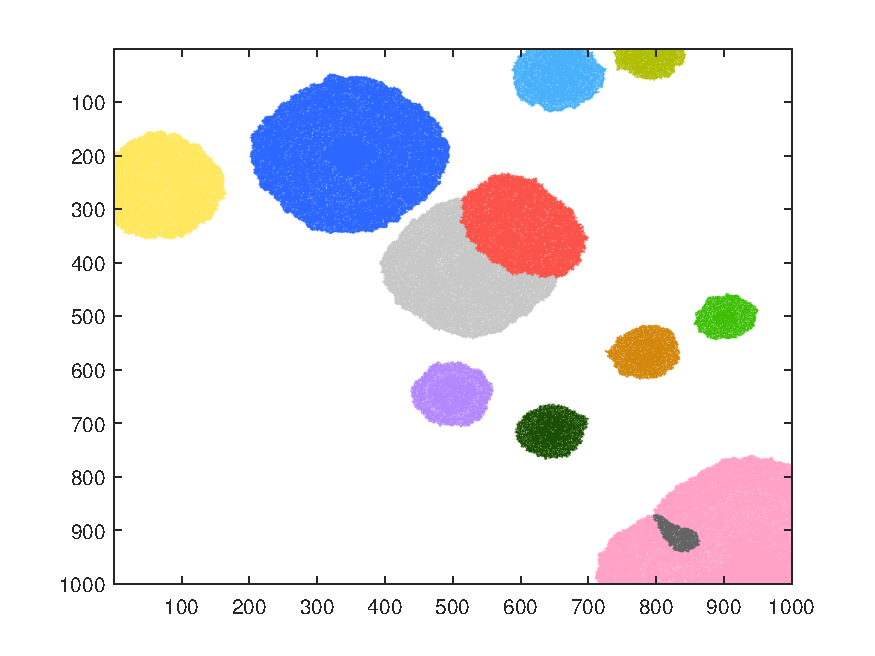
\includegraphics[width=\textwidth]{./picture/Eg_600day.pdf}
		\caption{Colony at t = 600 days}
		\label{Eg_colony600}
	\end{subfigure}
	\begin{subfigure}{0.3\textwidth}
			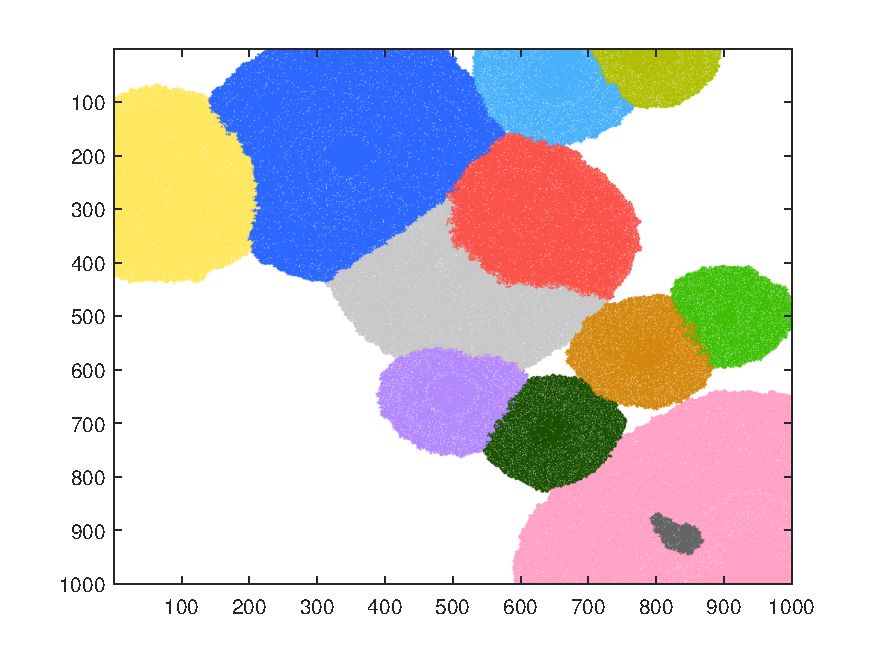
\includegraphics[width=\textwidth]{./picture/Eg_1500day.pdf}
			\caption{Colony at t = 1500 days}
			\label{Eg_colony1500}
	\end{subfigure}
	\begin{subfigure}{0.3\textwidth}
		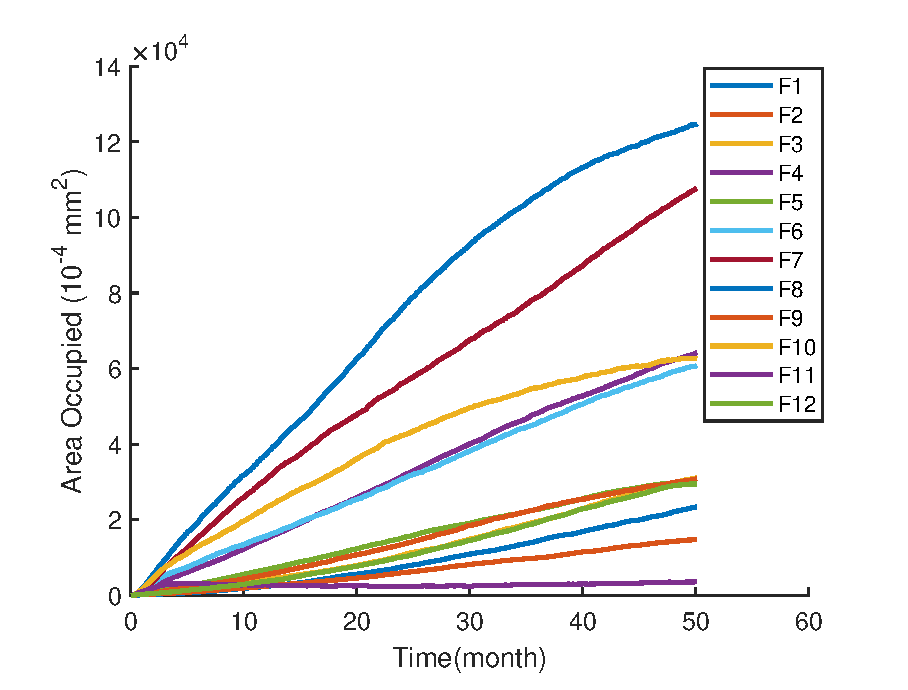
\includegraphics[width=\textwidth]{./picture/Eg_junsi.eps}
		\caption{Area occupied}
		\label{Eg_area}
	\end{subfigure}
	\begin{subfigure}{0.3\textwidth}
		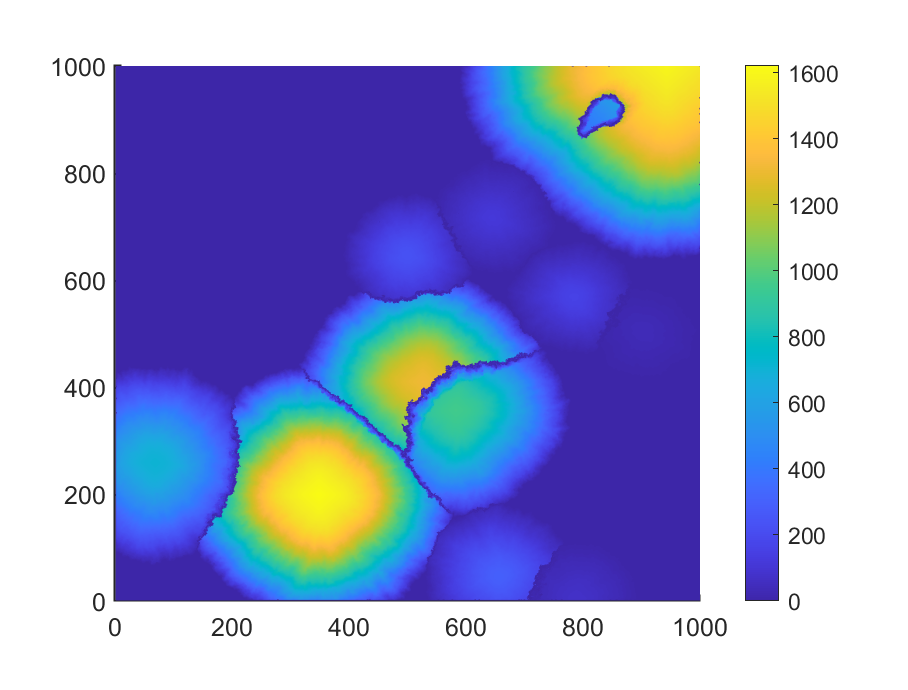
\includegraphics[width=\textwidth]{./picture/g_houduE.eps}
		\caption{Hyphal thickness}
		\label{Eg_thick}
	\end{subfigure}
	\begin{subfigure}{0.3\textwidth}
		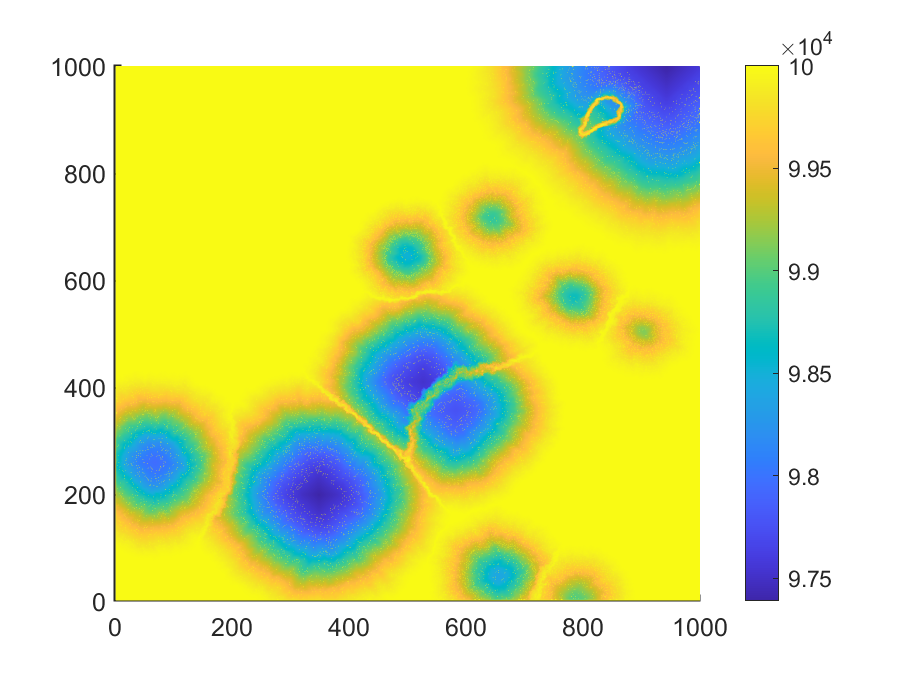
\includegraphics[width=\textwidth]{./picture/Eg_muban.eps}
		\caption{Thickness of wood left}
		\label{Eg_wood}
	\end{subfigure}
	\caption{The decomposition process and results ((c), (d), (e)) at the 1500th day.}
\end{figure}




\section{Analysis of Interactions}
\subsection{Fungi's Interactions without Environmental Changes}
Before considering the environmental factors, the model is first used to predict the interaction between two fungi under a relatively stable condition. A total of 12 species named F1 to F12 is chosen for testing with data obtained from Maynard's work on Nature \cite{Nature} and the results are concluded into short-term trends and long-term trends. The conclusion is used as a reference and comparison for the next part.

The conditions for \textit{2 vs 2} competition can be categorized into four types as follows. In each category, we choose a typical example for demonstration. (Note: Each pair is denoted as the combination of two names. For example, pair "F1F7" means the interaction between F1 and F7. "Boundary" means the line where the two colony meets.)

\begin{figure}[H]
	\centering
	\begin{subfigure}{0.3\textwidth}
		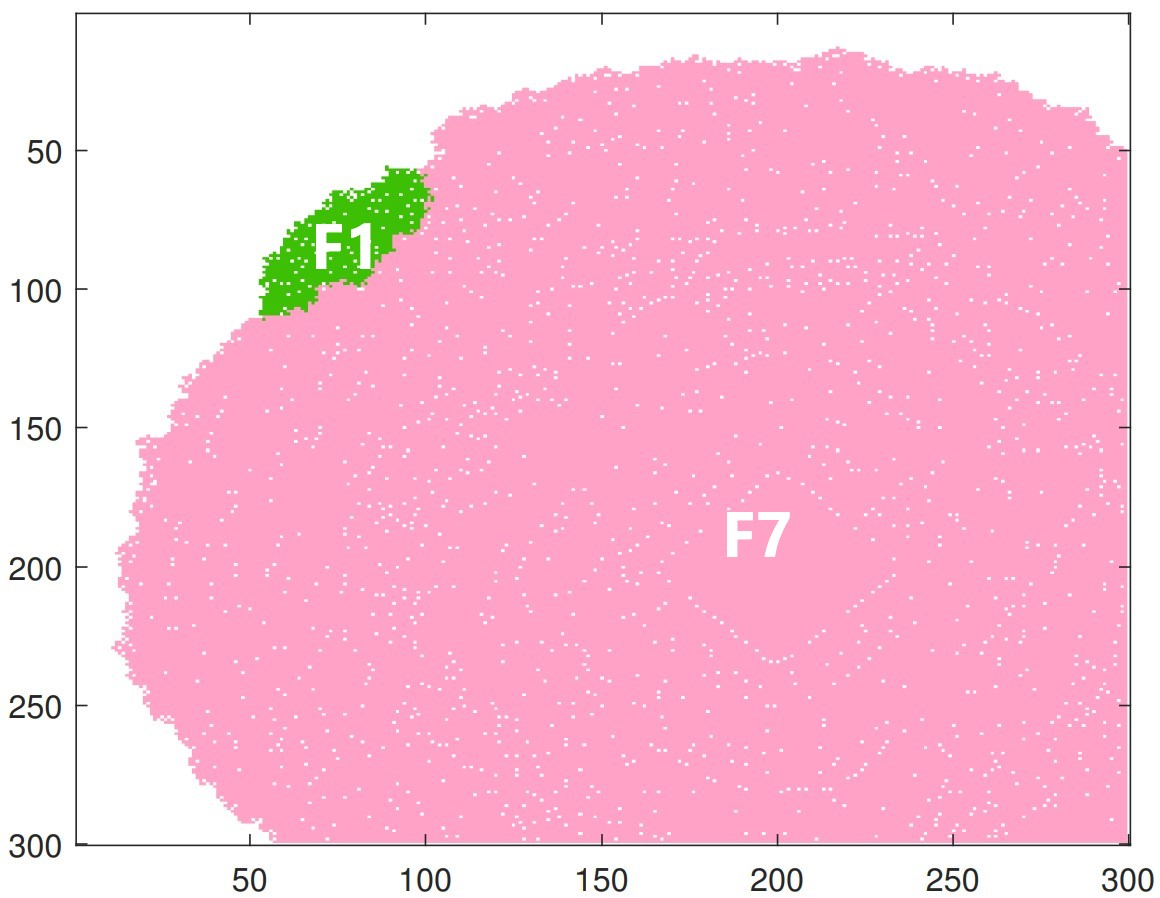
\includegraphics[width=\textwidth]{./4/noE_F1F7_650.jpg}
		\caption{Colony of F1F7 (Day 650)}
		\label{noE_F1F7_650}
	\end{subfigure}
	\begin{subfigure}{0.3\textwidth}
		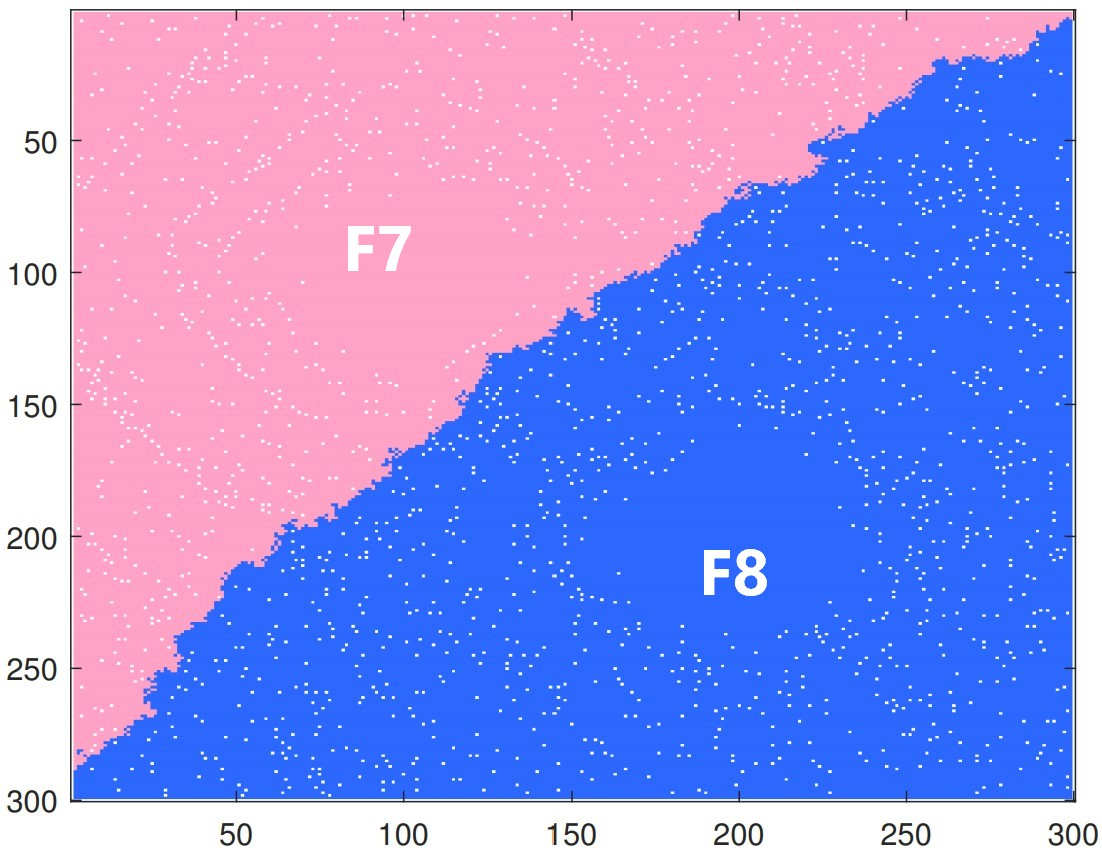
\includegraphics[width=\textwidth]{./4/noE_F7F8_860.jpg}
		\caption{Colony of F7F8 (Day 860)}
		\label{noE_F7F8_860}
	\end{subfigure}
	\begin{subfigure}{0.3\textwidth}
		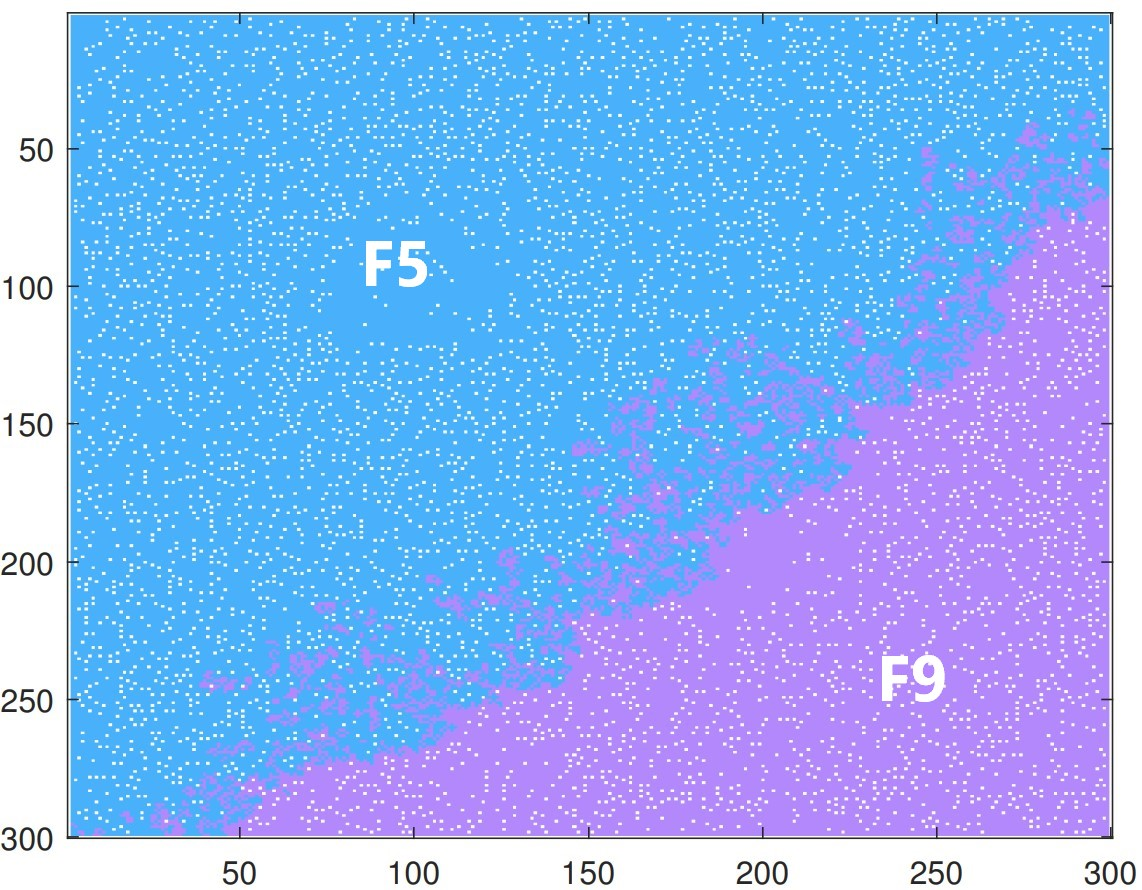
\includegraphics[width=\textwidth]{./4/noE_F5F9_4500.jpg}
		\caption{Colony of F5F9 (Day 4500)}
		\label{noE_F5F9_450}
	\end{subfigure}
	\caption{Colony of fungi (without environmental changes).}
	\end{figure}

\begin{enumerate}
\setlength{\itemsep}{0ex} %条目间距
\item \textbf{Overwhelming winning-losing} (Pair: F1F7; $E_7>>E_1$, $R_7>>R_1$)
\\\textit{Short-term}: F7 grows much faster than F1. As they meet, their boundary moves quickly towards F1 without deadlock, as shown in Fig.~\ref{noE_F1F7_650}.
\\\textit{Long-term}: F7 coves F1 totally and occupies the whole area.
\item \textbf{Quickly determined winning-losing} (Pair: F4F7; $E_7>E_4$, $R_7>R_4$)
\\\textit{Short-term}: F7 grows faster than F4. Some degrees of deadlock at the boundary.
\\\textit{Long-term}: Winning-losing is quickly determined and F4 is driven out.
\item \textbf{Deuce at first} (Pair: F7F8; $E_8\approx E_7$, $R_8>R_7$)
\\\textit{Short-term}: The boundary is formed at the diagonal as shown in Fig.~\ref{noE_F7F8_860}. No obvious trend of winning-losing.
\\\textit{Long-term}: F8 gradually drives out F7, with a clear boundary in the process.
\item \textbf{Long-run Competition} (Pair: F5F9; $E_5\approx E_9$, $R_5 \approx R_9$)
\\\textit{Short-term}: The boundary is formed at the diagonal. No obvious trend of winning-losing.
\\\textit{Long-term}: The competition lasts for a very long time and F5 previals slowly. There is obvious deadlock at the boundary, as shown in Fig.~\ref{noE_F5F9_4500}.
\end{enumerate}
The following four figures are the plots of areas occupied by each fungus with respect to time, which reflects the four conditions mentioned above. 

\vspace{-0.3cm}
\begin{figure}[H]
%\captionsetup{font={footnotesize}}
\centering 
\begin{subfigure}{0.4\textwidth}
	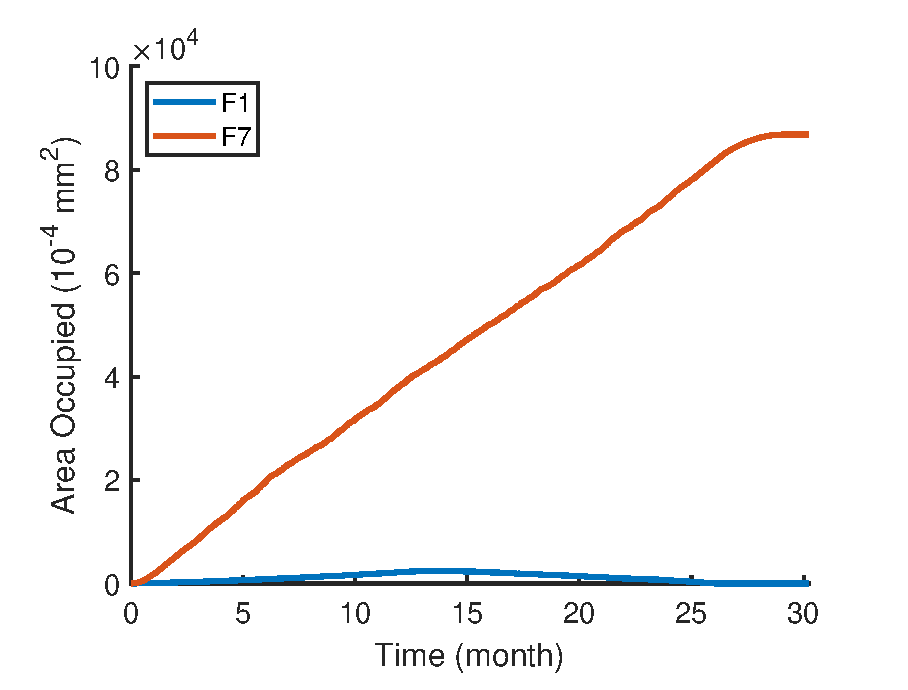
\includegraphics[width=\textwidth]{./4/noE_F1F7_area.eps}
	\caption{(F1F7)}
	\label{noE_F1F7_area}
\end{subfigure}
\begin{subfigure}{0.4\textwidth}
	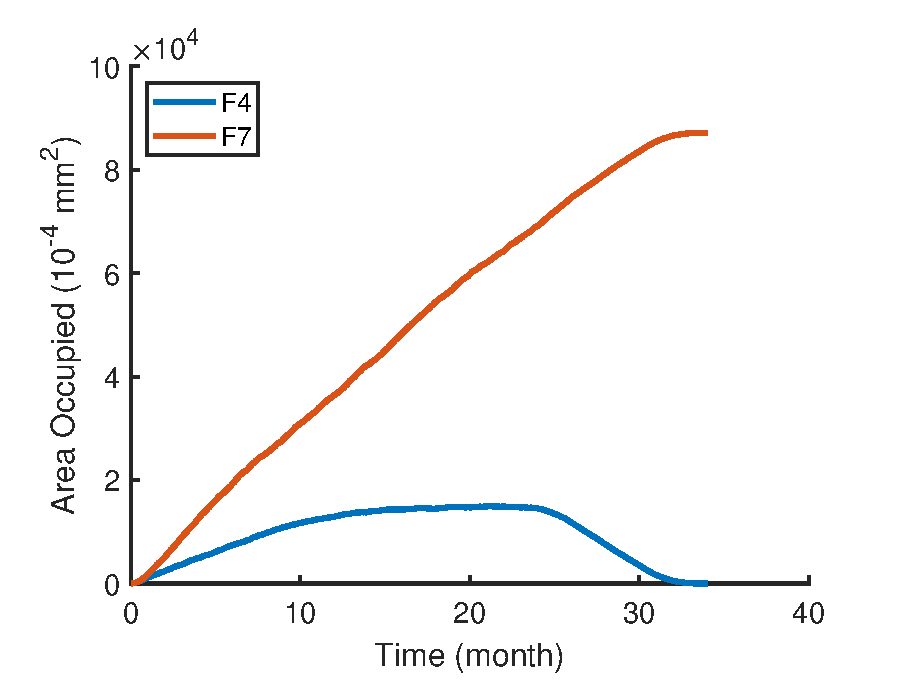
\includegraphics[width=\textwidth]{./4/noE_F4F7_area.eps}
	\caption{(F4F7)}
	\label{noE_F4F7_area}
\end{subfigure}
\begin{subfigure}{0.4\textwidth}
	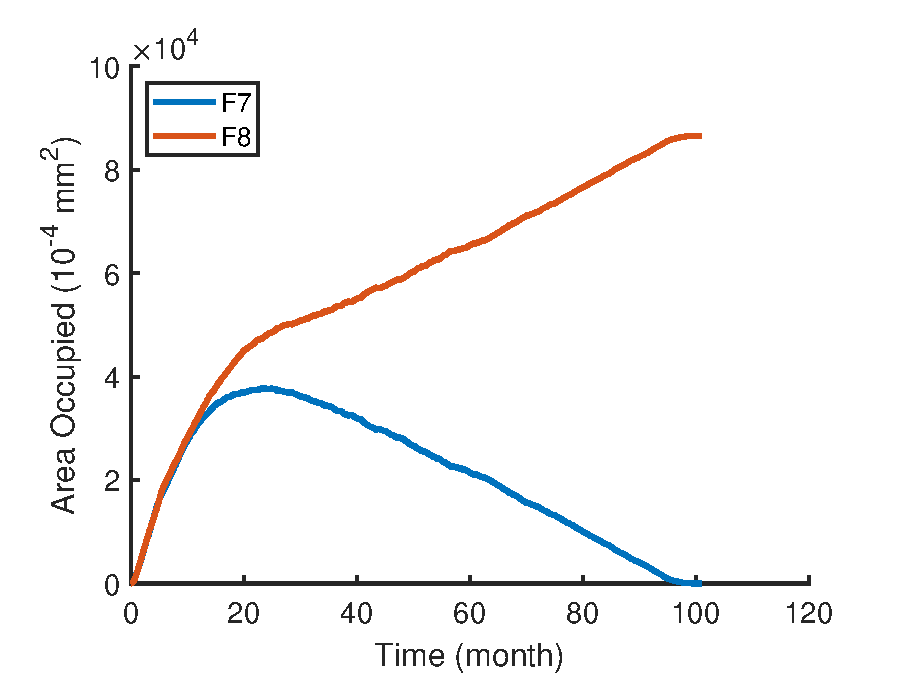
\includegraphics[width=\textwidth]{./4/noE_F7F8_area_2.eps}
	\caption{(F7F8)}
	\label{noE_F7F8_area}
\end{subfigure}
\begin{subfigure}{0.4\textwidth}
	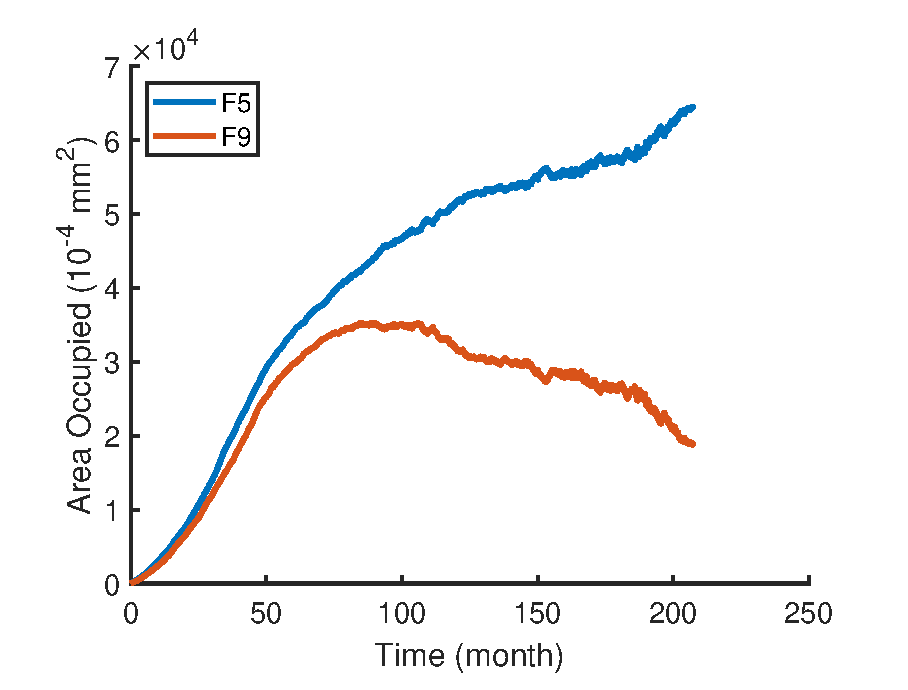
\includegraphics[width=\textwidth]{./4/noE_F5F9_area.eps}
	\caption{(F5F9)}
	\label{noE_F5F9_area}
\end{subfigure}
\caption{Area occupied by fungi in different interactions (without environmental changes).}
\label{noE_area}
\end{figure}


\subsection{Changing Atmospheric Conditions: Temperature and Moisture}
\par To analyze the trends of interaction in a long time, the changing of environmental conditions must be taken into consideration. To simulate the changing of weather patterns in a year, we find the data of monthly temperature and precipitation in Boston in 2020, as shown in Fig.~\ref{weather} \cite{weather}. 

\begin{figure}[H]
	\centering
	\begin{subfigure}{0.44\textwidth}
		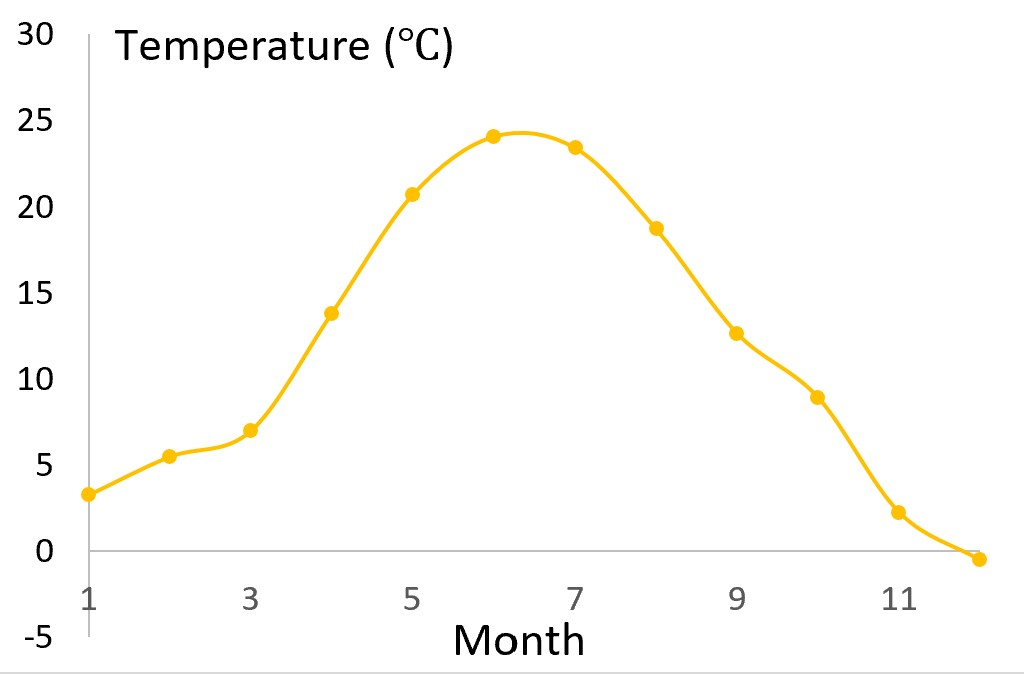
\includegraphics[width=\textwidth]{./4/temp.jpg}
	\end{subfigure}
	\begin{subfigure}{0.45\textwidth}
		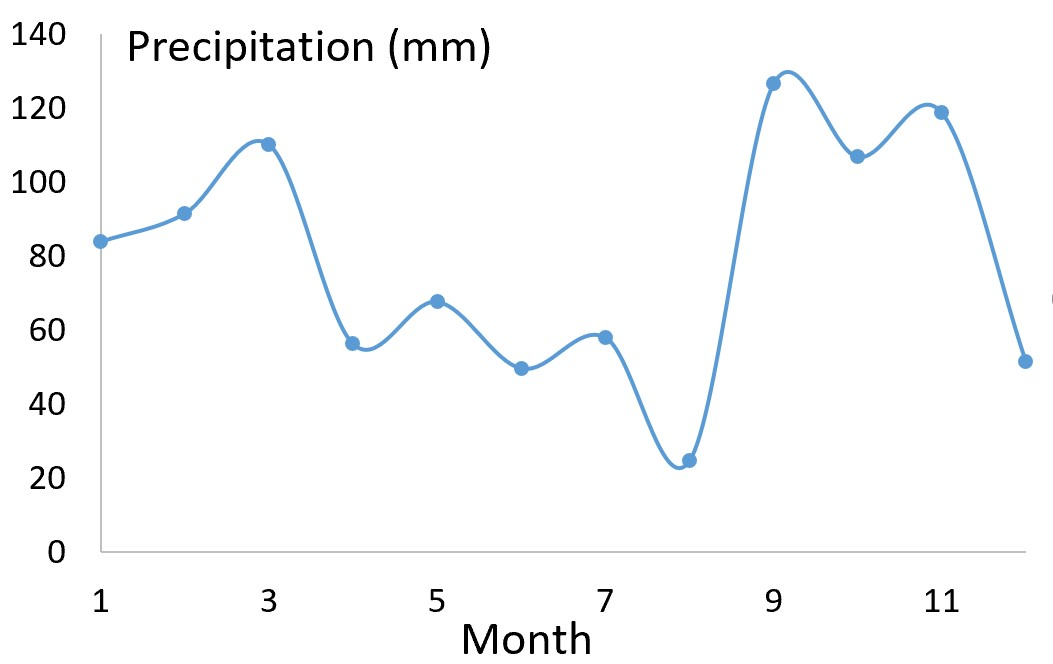
\includegraphics[width=\textwidth]{./4/precipitation.jpg}
	\end{subfigure}
	\caption{Monthly Average Temperature and Precipitation in Boston, 2020 \cite{weather}.}
	\label{weather}
\end{figure}
\vspace{-0.2cm}
\par We approximate the moisture by scaling the precipitations into values between 0.08 and 5.25, because no direct information of moisture is found and the trends of moisture and precipitation should be very close to each other, according to literature \cite{mois-pre}. Then we fit the data into functions, as the expressions of temperature $T$ and moisture $m$. Eqn.~\eqref{temp} is the temperature function of time t (the moisture function is more complicated and not listed here). 

\begin{equation}
	\label{temp}
	T=12.3 \cos (\frac{2\pi}{365}t-\frac{\pi}{2})+11.75
\end{equation}

If we denote $[m_{min},m_{max}]$ as $I_m$ and $[T_{min},T_{max}]$ as $I_T$, the expression of hyphal extension rate now becomes:
\begin{eqnarray}
	E=
	\begin{cases}
		E_0 & m \in I_m, T\in I_T\\
		E_0\times e^{-\min\{\vert m-m_{min} \vert, \vert m-m_{max} \vert\}} & m \notin I_m, T\in I_T\\
		E_0\times e^{-0.1\min\{\vert T-T_{min} \vert, \vert T-T_{max} \vert\}} & m \in I_m, T\notin I_T\\
		E_0\times e^{-\min\{\vert m-m_{min} \vert, \vert m-m_{max} \vert\}} \times e^{-0.1\min\{\vert T-T_{min} \vert, \vert T-T_{max} \vert\}} & m \notin I_m, T\notin I_T\\
	\end{cases}
\end{eqnarray}

\subsection{Interactions between Fungi with Environmental Changes}
\par In order to show how the environmental conditions influence the interactions of fungi, we choose the same four pairs of fungi as in Section \ref{sec3.1} for analysis. The area-time plots are shown in Fig.~\ref{E_area}. Comparing with Fig.~\ref{noE_area}, the interactions with environmental changes show some different trends, which are going to be discussed next.

\begin{figure}[H]
	%\captionsetup{font={footnotesize}}
	\centering 
	\begin{subfigure}{0.4\textwidth}
		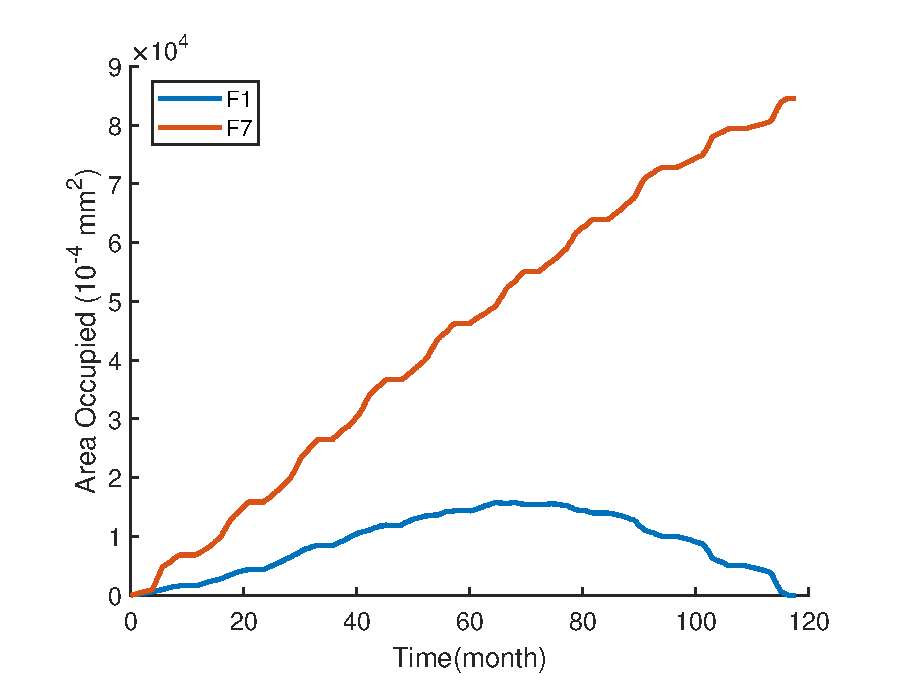
\includegraphics[width=\textwidth]{./4/E_F1F7_area.eps}
		\caption{(F1F7)}
		\label{E_F1F7_area}
	\end{subfigure}
	\begin{subfigure}{0.4\textwidth}
		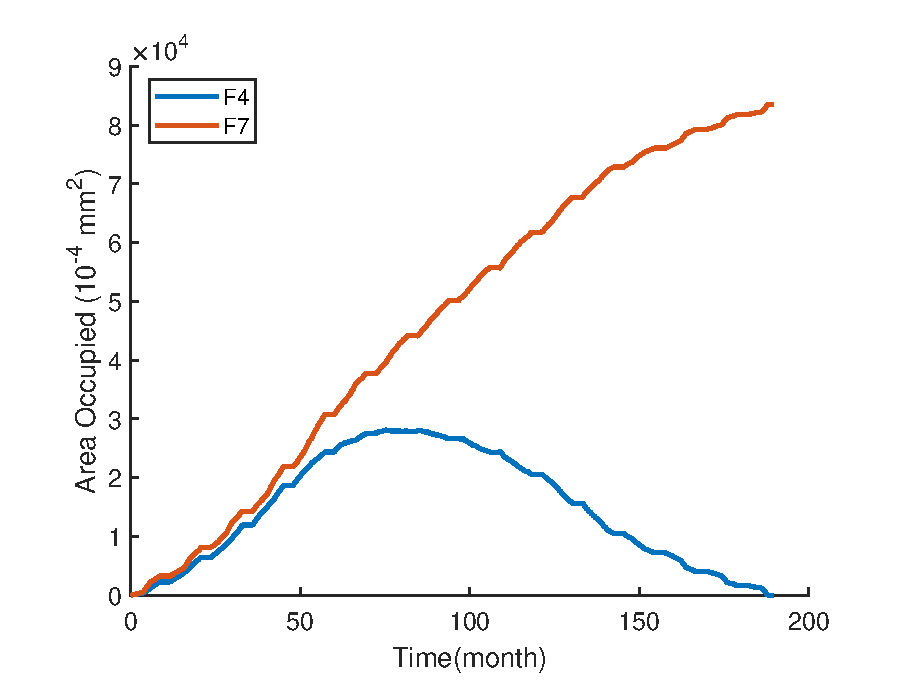
\includegraphics[width=\textwidth]{./4/E_F4F7_area.eps}
		\caption{(F4F7)}
		\label{E_F4F7_area}
	\end{subfigure}
	\begin{subfigure}{0.4\textwidth}
		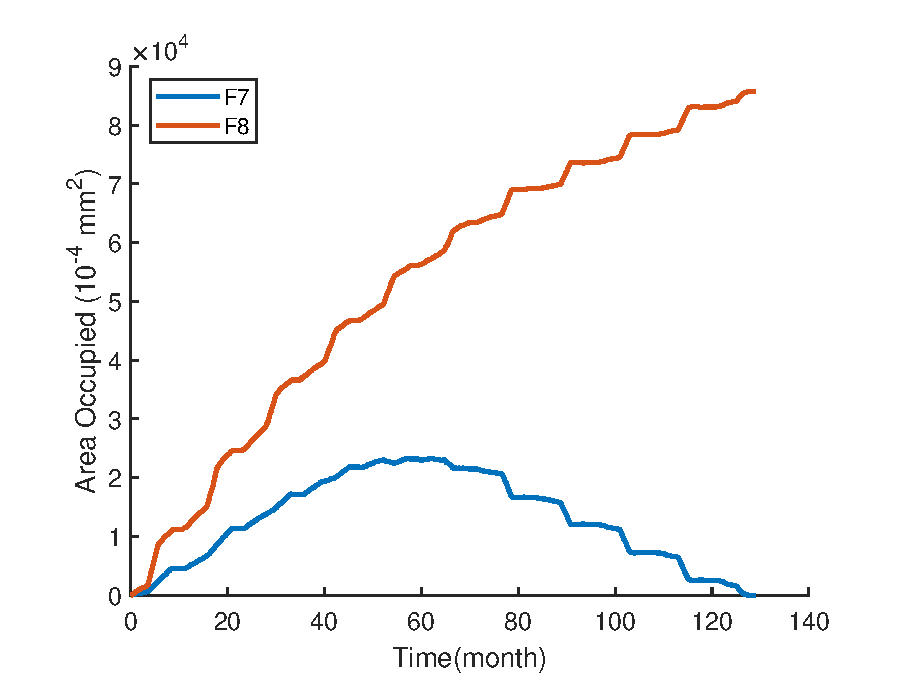
\includegraphics[width=\textwidth]{./4/E_F7F8_area.eps}
		\caption{(F7F8)}
		\label{E_F7F8_area}
	\end{subfigure}
	\begin{subfigure}{0.4\textwidth}
		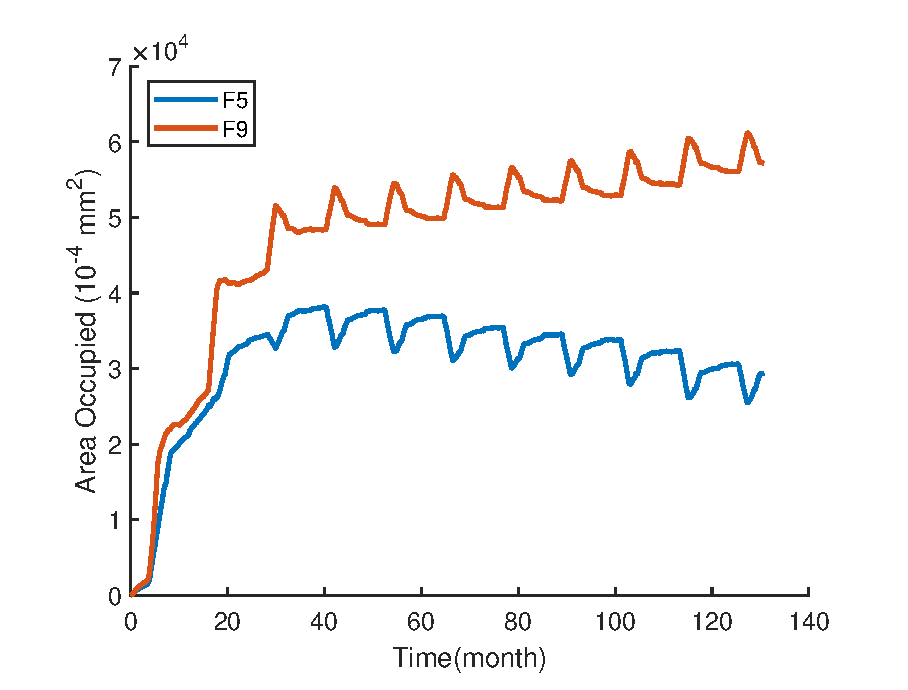
\includegraphics[width=\textwidth]{./4/E_F5F9_area_2.eps}
		\caption{(F5F9)}
		\label{E_F5F9_area}
	\end{subfigure}
	\caption{Area occupied by fungi in interactions (with atmosphere trends changing).}
	\label{E_area}
	\end{figure}

\par Firstly, the area-time curves in Fig.~\ref{E_area} are \textbf{no longer smooth} as in Fig.~\ref{noE_area}. Instead, there are periodical dentate fluctuations on the curves. This is a result of the changing temperature and moisture in each year. Another phenomenon reflecting the annual changes is the "growth rings" on the colonies, as shown in Fig.~\ref{E_colony} (especially on the colony of F8). When the temperature and moisture are suitable, the fungi grow faster and the hyphae look sparser; and when the conditions are unsuitable, the hyphae look denser. 

	\begin{figure}[H]
		%\captionsetup{font={footnotesize}}
		\centering 
		%\begin{subfigure}{0.3\textwidth}
		%	\includegraphics[width=\textwidth]{E_F1F7_1800.jpg}
		%	\caption{Colony of F1F7 (Day 1800)}
		%	\label{E_F1F7_1800}
		%\end{subfigure}
		\begin{subfigure}{0.3\textwidth}
			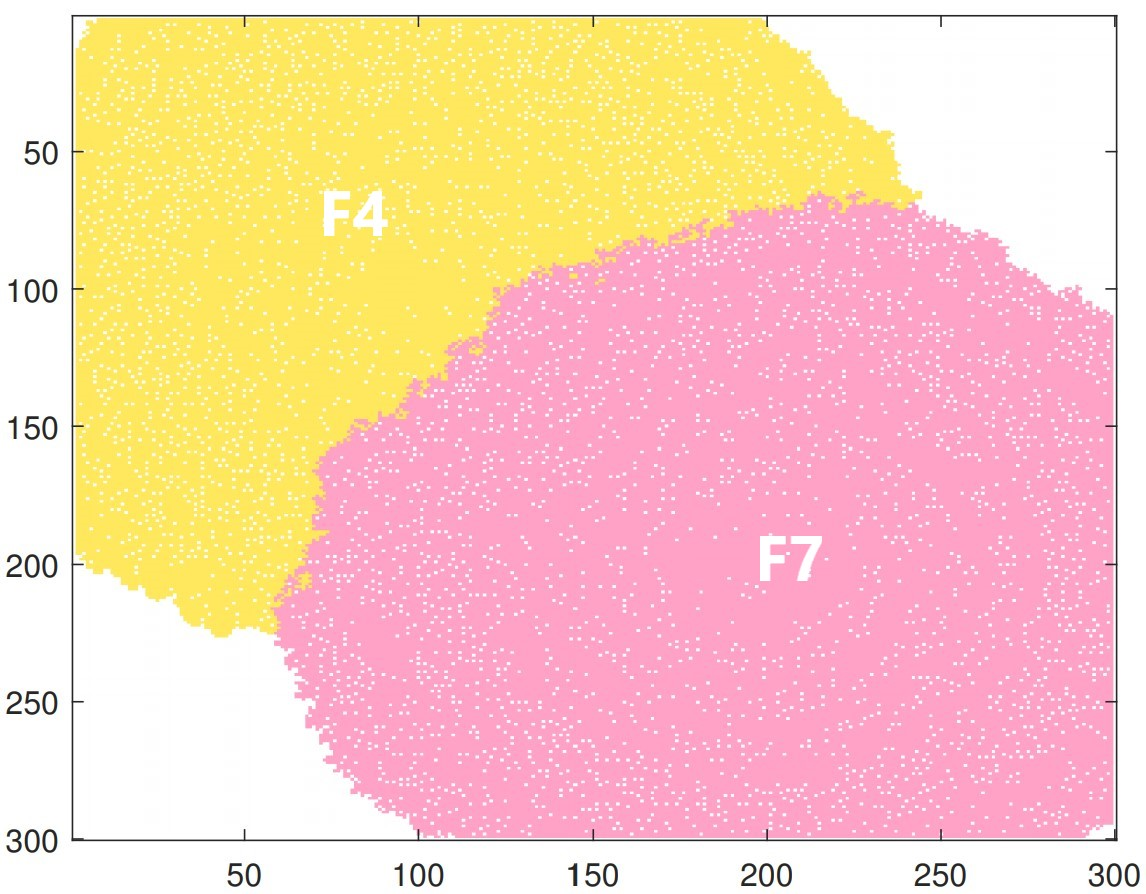
\includegraphics[width=\textwidth]{./4/E_F4F7_2500.jpg}
			\caption{Colony of F4F7 (Day 2500)}
			\label{E_F4F7_2500}
		\end{subfigure}
		\begin{subfigure}{0.3\textwidth}
			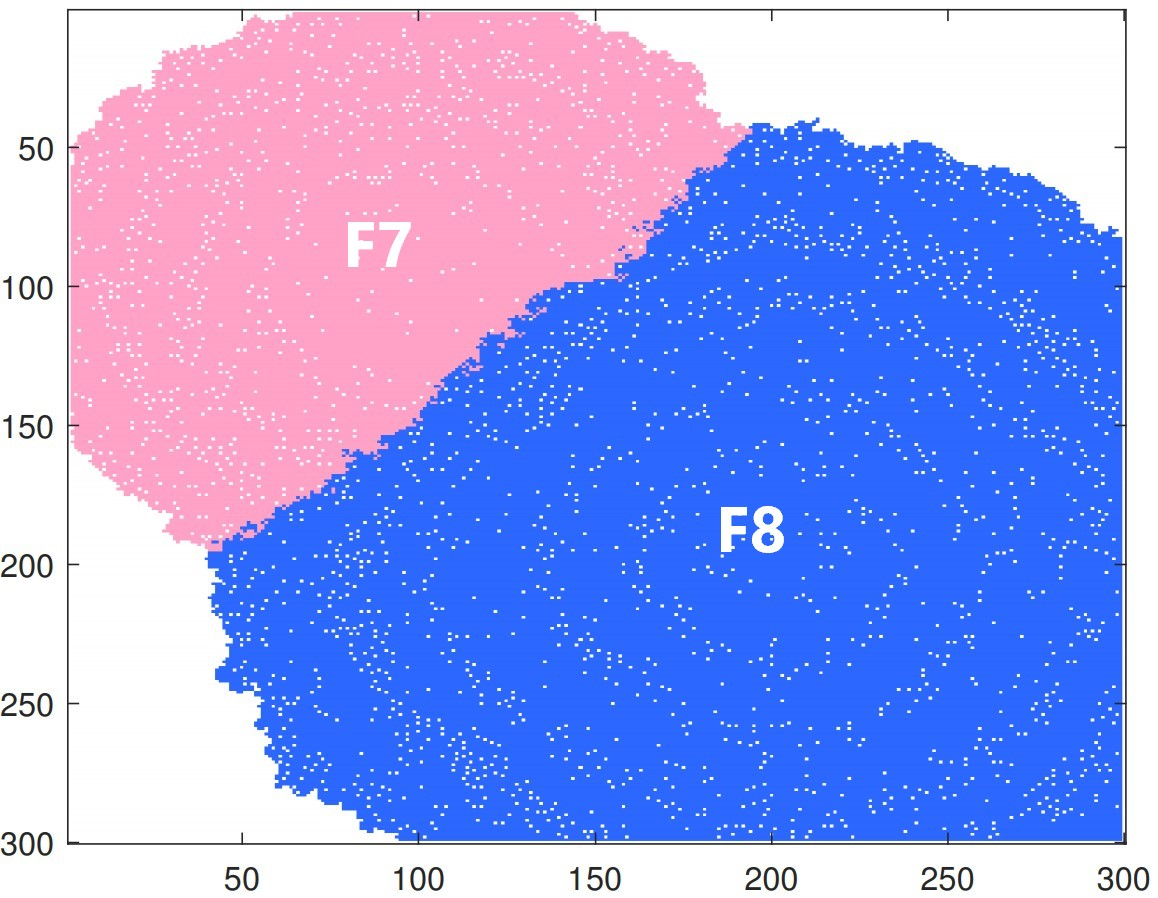
\includegraphics[width=\textwidth]{./4/E_F7F8_1550.jpg}
			\caption{Colony of F7F8 (Day 1550)}
			\label{E_F7F8_1550}
		\end{subfigure}
		\begin{subfigure}{0.3\textwidth}
			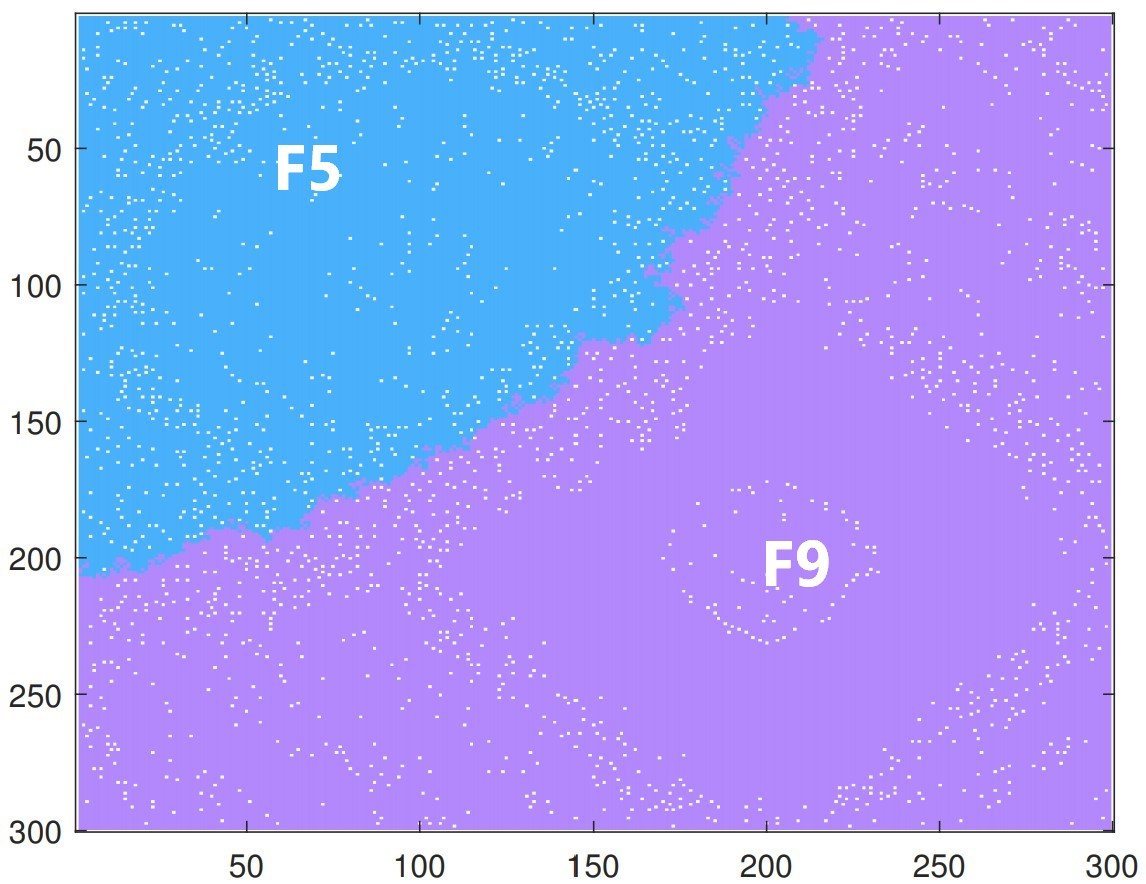
\includegraphics[width=\textwidth]{./4/E_F5F9_3920.jpg}
			\caption{Colony of F5F9 (Day 3920)}
			\label{E_F5F9_3920}
		\end{subfigure}
		\caption{Colony of fungi (with atmosphere trends changing).}
		\label{E_colony}
		\end{figure}

\par Secondly, the \textbf{"overwhelming winning-losing" condition disappears}. In pair F1F7, the weaker fungus F7 exists for a longer time than before, and the maximum area it occupies also increases. The similar thing also happens to F4F7. The explanation is, the preponderance of F7 is weaken when the environment is changing because of its low tolerance to different temperature and moisture conditions.
\par Thirdly, \textbf{the competition result in a pair can even be reversed}. Comparing Fig.~\ref{E_F5F9_area} with Fig.~\ref{noE_F5F9_area}, and Fig.~\ref{E_F5F9_3920} with Fig.~\ref{noE_F5F9_4500}, we can see that the previaling fungus turns from F5 to F9. This is because F9 can adapt the temperature changes better. Besides, the competition between F5 and F9 becomes a "seesaw battle" when the environmental conditions change regularly.
\par Another thing to notice is that, in Fig.~\ref{E_colony}, the orientations of boundaries are different. The orientation of boundaries reflects the relative preponderance of competitiveness and growth rate. For example, in Fig.~\ref{E_F4F7_2500}, the boundary bulges to F4, which is in the direction of its movement. This indicates that F7 wins F4 mainly by high competitiveness (ranking). In Fig.~\ref{E_F5F9_3920}, the boundary is concave with respect to its moving direction, which indicates that F9 wins F5 mainly by high growth rate.

\subsection{Impact of Rapid Fluctuations in External Environment}
In order to study the impact of rapid environmental fluctuations on the interaction of fungi, we firstly simulate an environment with fluctuating temperature and moisture, as shown in Fig.~\ref{fluctuation}. The fluctuations are created by randomizing the values every five days.
\begin{figure}[H]
	\centering
	\begin{subfigure}{0.42\textwidth}
		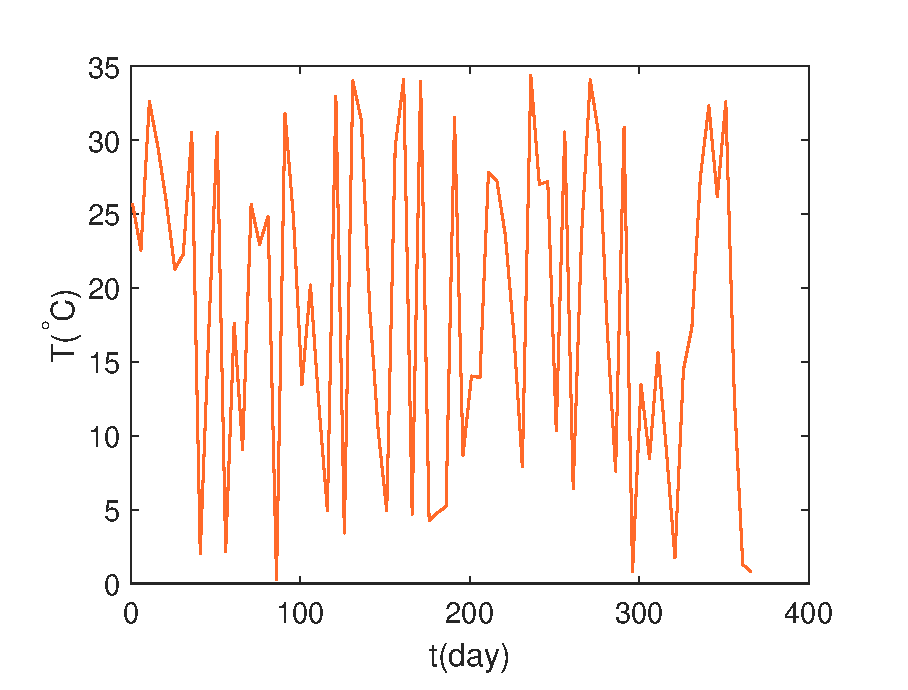
\includegraphics[width=\textwidth]{./4/T_fluc.eps}
	\end{subfigure}
	\begin{subfigure}{0.42\textwidth}
		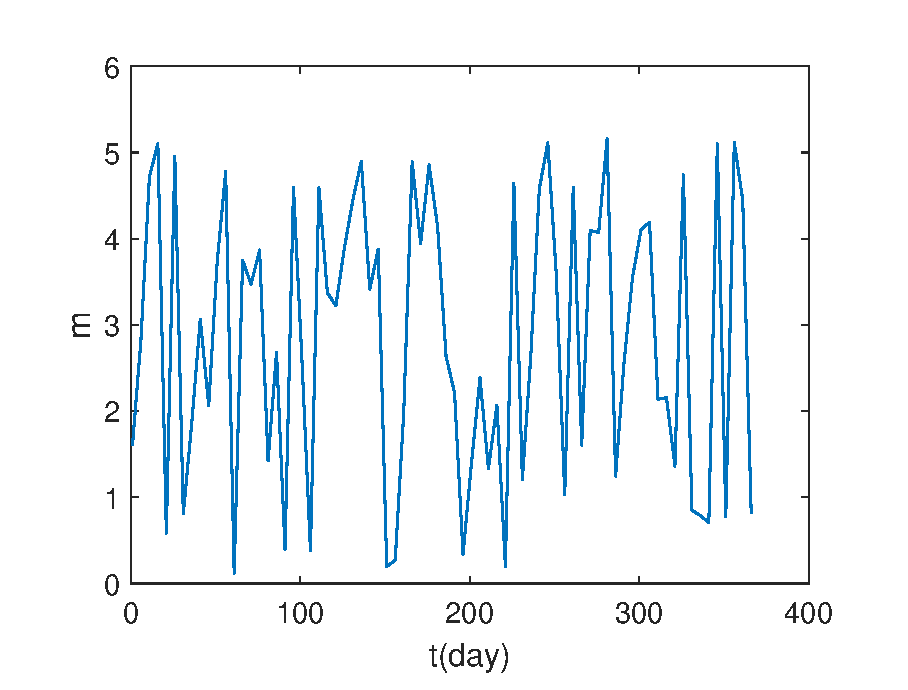
\includegraphics[width=\textwidth]{./4/m_fluc.eps}
	\end{subfigure}
	\caption{Patterns of rapid fluctuations in temperature $T$ and moisture $m$.}
	\label{fluctuation}
\end{figure}

\par Then the celluar automata model will be used to simulate how a single fungus grow under random and rapid environmental changes. Documentation claims that the hyphae of fungi that can better adapt to the environment are denser and expand more slowly \cite[CompArticle], so will they have high adaptability in this random environment? We mainly measure the change of the surface area of a fungus on 100[mm] $\times$ 100 [mm] wood blocks. It will expand from the center until covering the whole block. Fig.\eqref{sjsjsj} shows the process and area change curve for 12 different fungi under 5 different random conditions.
\begin{figure}[H]
	\centering
	\begin{subfigure}{0.45\textwidth}
		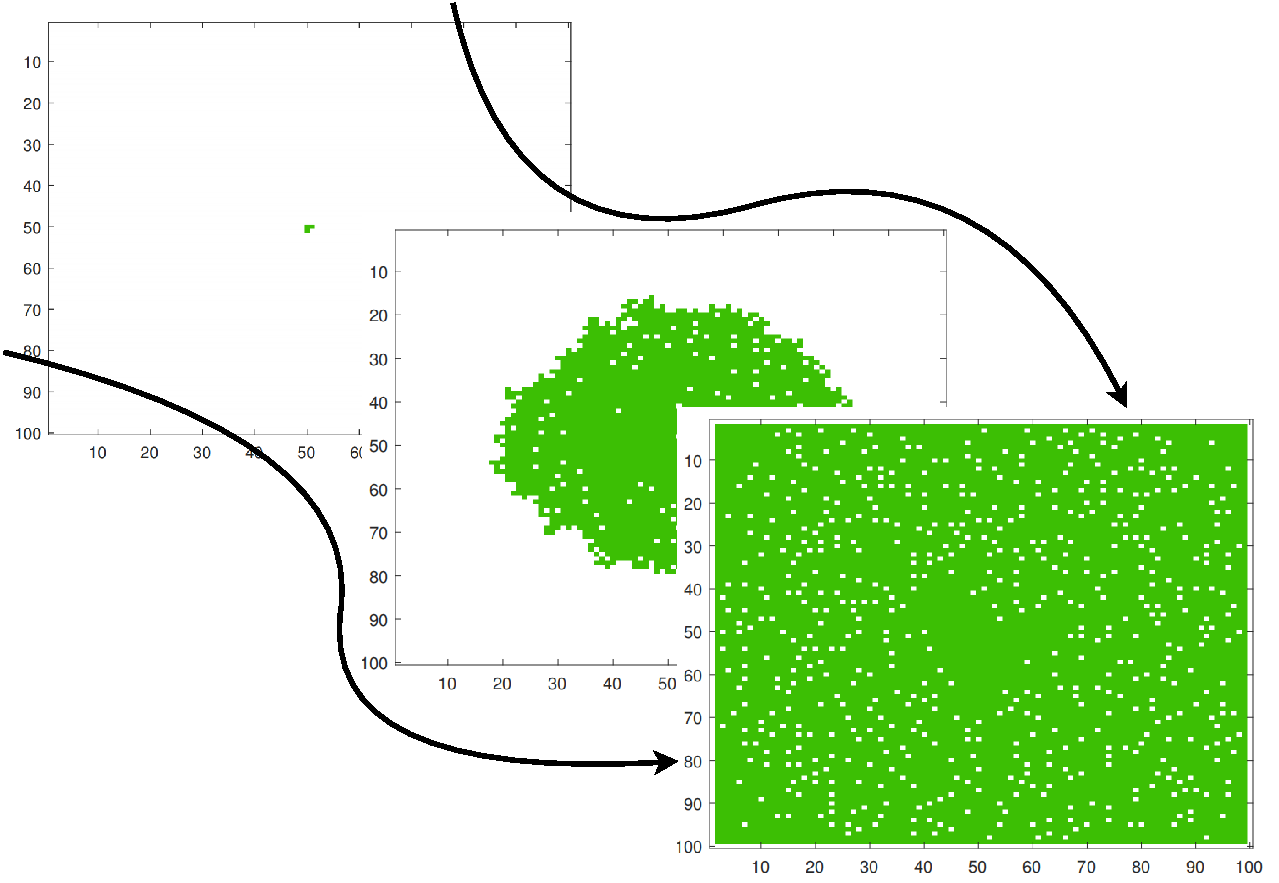
\includegraphics[width=\textwidth]{./picture/SJflow.pdf}
	\end{subfigure}
	\begin{subfigure}{0.45\textwidth}
		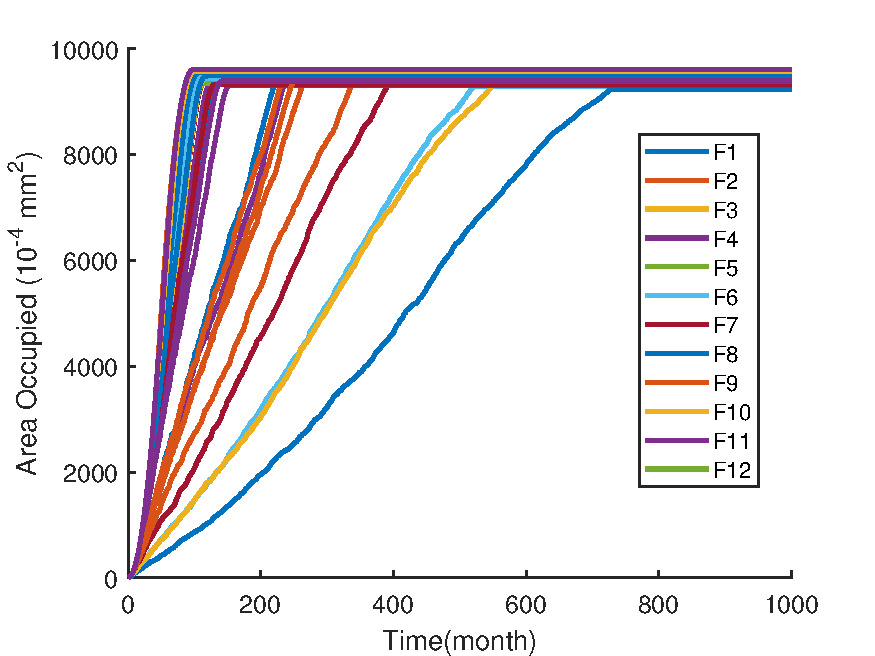
\includegraphics[width=\textwidth]{./picture/12for5.pdf}
	\end{subfigure}
	\caption{Tset process and results for rapid fluctuations in $T$ and $m$.}
	\label{sjsjsj}
\end{figure}

From the Fig.\eqref{sjsjsj}, we can find that some color curve families, such as F3-orange curve family, do not deviate too much from each other and almost grow in the same trend, while some color curve families, such as blue-F8 curve family in, deviate much from each other. This is because fungi like F3 have a higher moisture niche width and temperature niche widt so when they face the fluctuation of the environment, their range of change is smaller which means that they are more \textbf{stable}.
\begin{figure}[H] 
	\centering 
	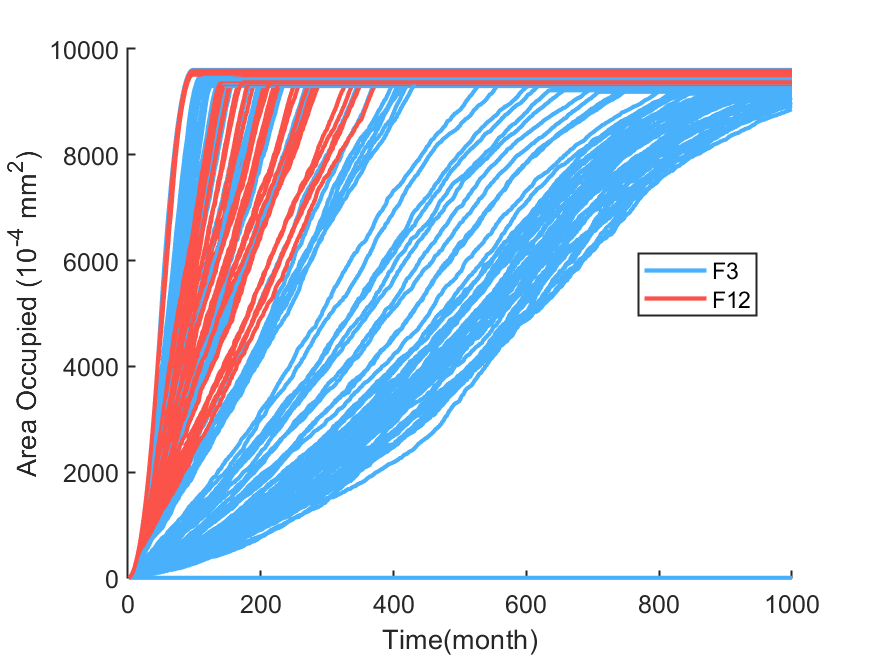
\includegraphics[height=6cm]{./picture/3vs12.pdf}
	\caption{Area change curves of F3 and F12 (50 for each).}
	\label{spspsp}
\end{figure}
\par Also, this kind of stability will also affect the speed of expension. For example, the expension speed of F12 fungi is 0.77 mm/day while the expension speed of F3 is greater than F12 which is 1.09 mm/day. However on Fig.\eqref{spspsp}, we repeat the simulation 50 times for F3 and F12 and can conclude that the average expantion speed of F12 is far more than F3 which means that those kind of fungi that are more stable will also have \textbf{advantage on expansion speed} when facing great change on emvironment. 


\section{Fungi Communities in different Environment}
In this part, predictions about the relative advantages and disadvantages for each species and combinations of species likely to persist are made using the previous designed model. Figure \ref{climate} shows the temperature and precipitation of five different climates under which we tested the vitality of our fungi. In order to select the best combinations, we've come up with one efficient way after real testing. One detailed example (tropical rain forest) is written down to demonstrate the process and the other four are only presented with a summarized result including advantages and disadvantages for each fungus as well as some possible combinations due to the page limit.
\vspace{-0.6cm}
\begin{figure}[H]
	\centering
	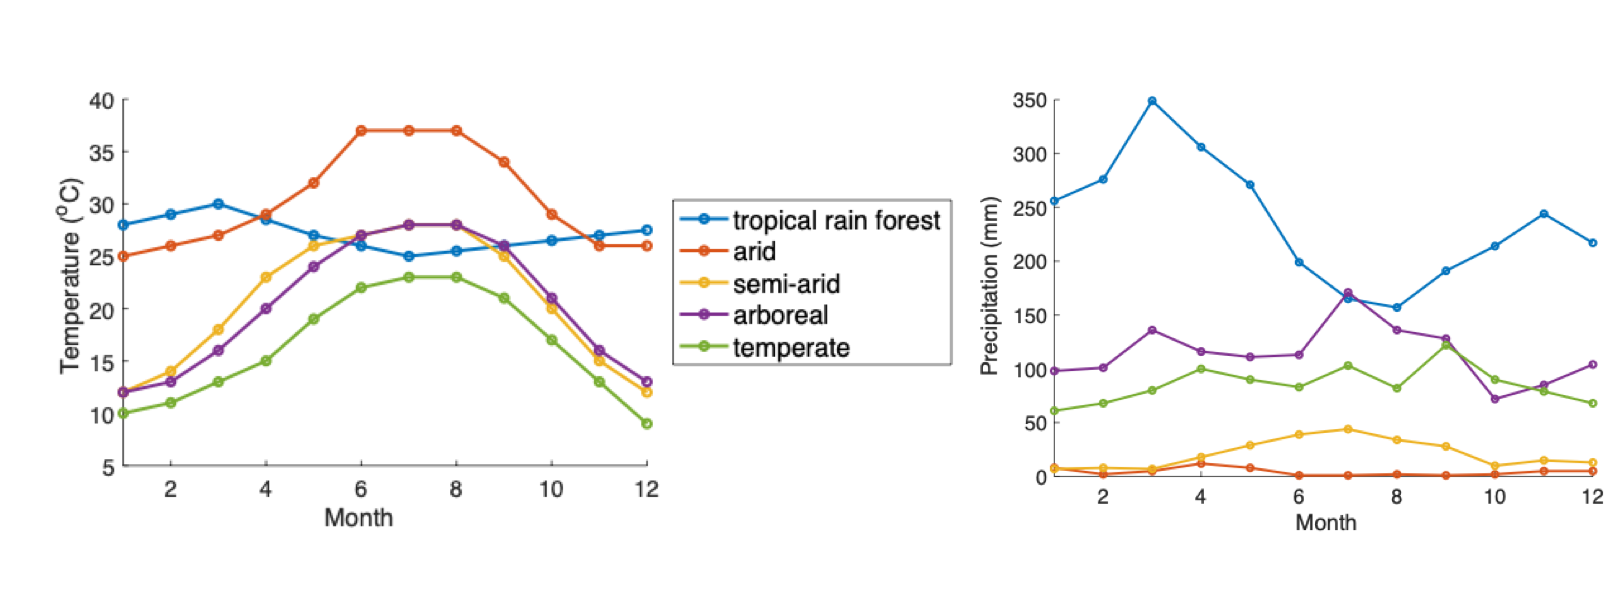
\includegraphics[height=6cm]{./figures/five.png}
	\caption{Temperature and precipitation of five climates. \cite{climate,climate2,arboreal,ocean}}
	\vspace{-0.3cm}
	\label{climate}
\end{figure}
 

\subsection{Example: Tropical Rain Forest}
Tropical rain forest climate has a relatively high temperature of 25-30 and a precipitation of >200 mm per month throughout the whole year. Thus, we first test the yearly performance of each fungus' growth. In order to first let them grow freely with less interaction between species, the testing is break up into three groups: F1-F5,F6 \& F9-F12, F7 \& F8, due to the fast growth of F7 and F8.The result is shown in Fig. \ref{F1-5} to Fig. \ref{F78}.

\begin{figure}[H]
\captionsetup{font={small}}
	\begin{minipage}{30ex}
	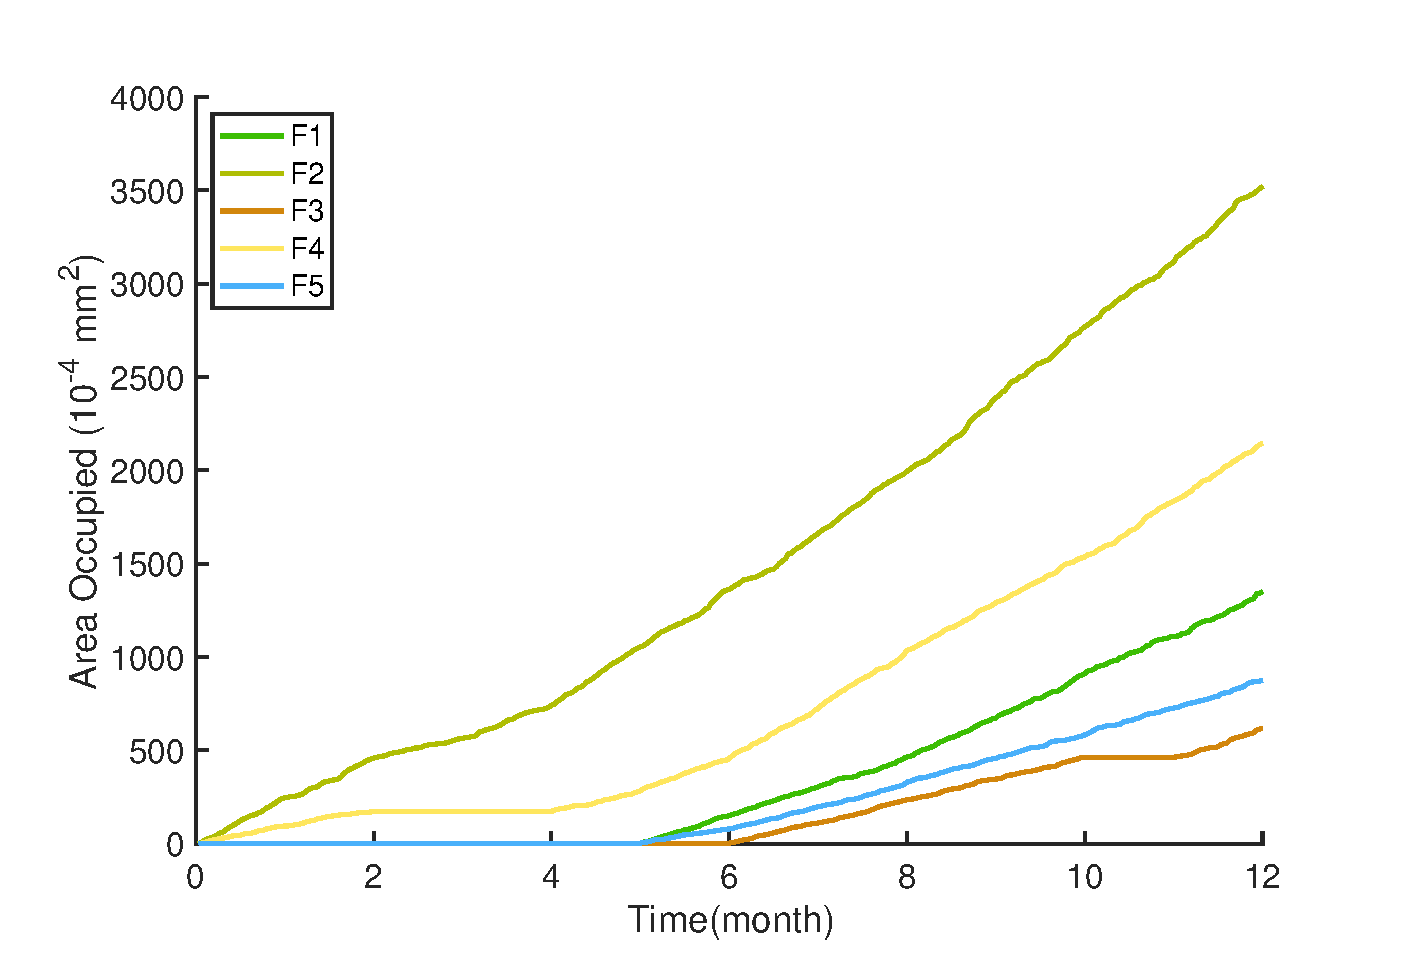
\includegraphics[height=4cm]{./formal/tropical/1-5.eps}
	\caption{Yearly growth of F1-5.}
	\label{F1-5}
\end{minipage}   
\begin{minipage}{30.5ex}
\centering
	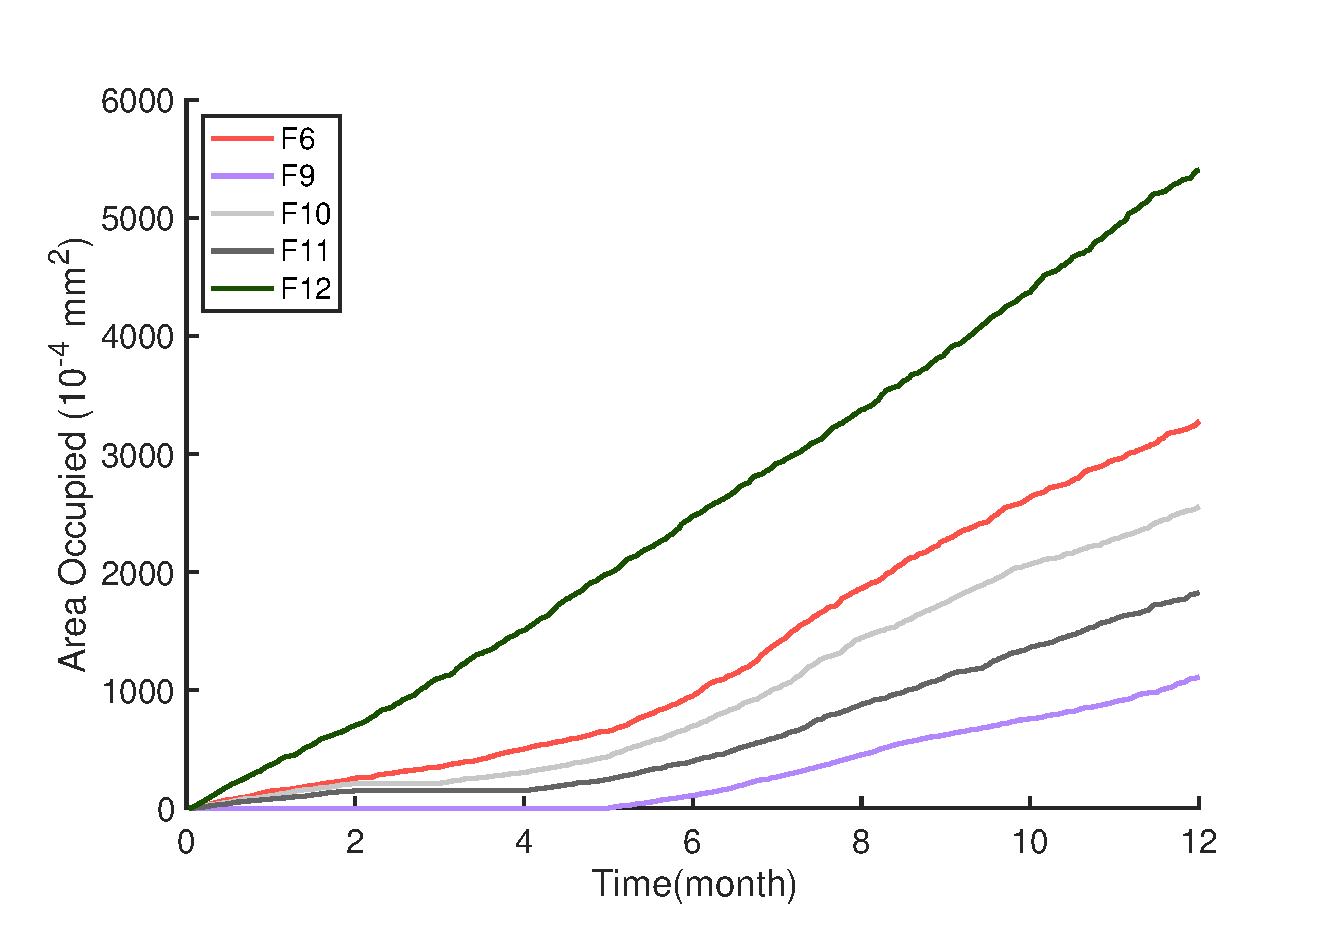
\includegraphics[height=4cm]{./formal/tropical/6&9-12.eps}
	\caption{Yearly growth of F6,9-12.}
	\label{F6}
\end{minipage}
\begin{minipage}{29ex}
\centering
	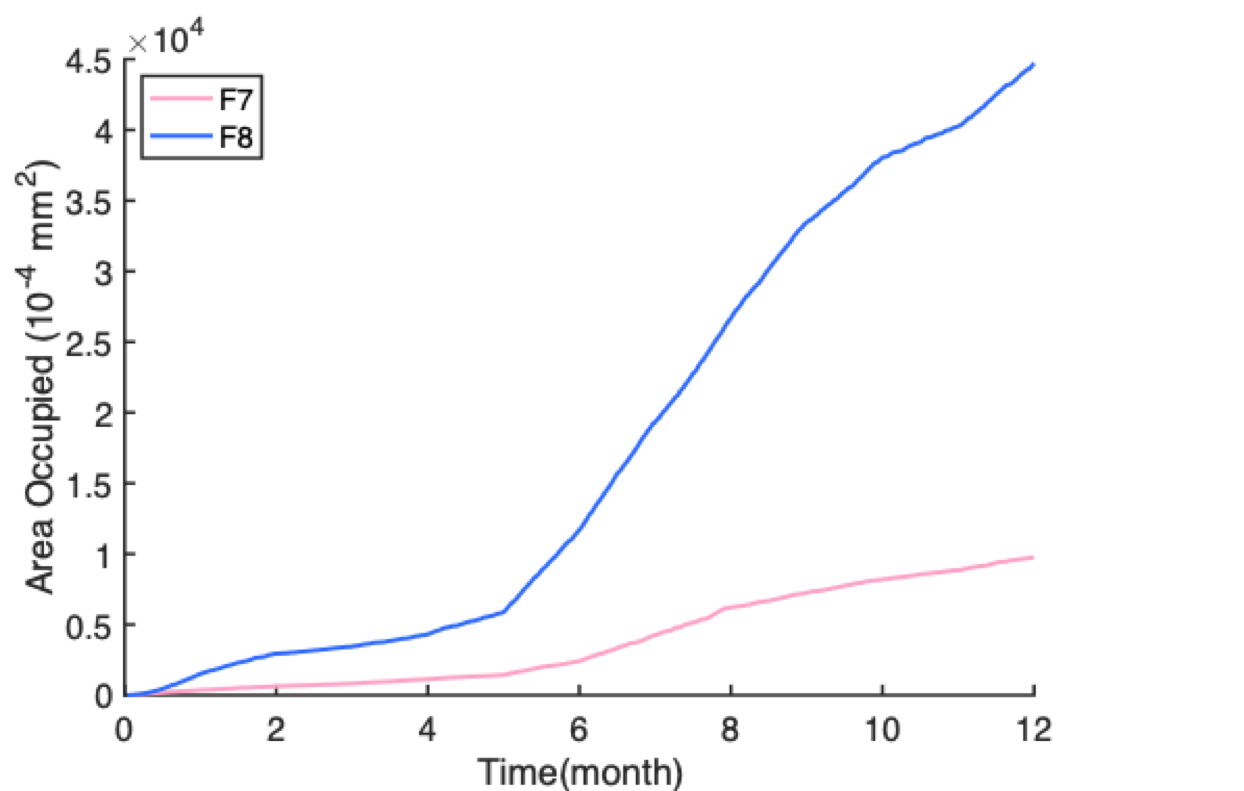
\includegraphics[height=4cm]{./formal/tropical/78.png}
	\caption{Yearly growth of F7 \& 8.}
	\label{F78}
\end{minipage} 
\end{figure}

Then we can conclude the effect of annual temperature and precipitation change on all 12 fungi and analyze their advantage and disadvantage according to the similarity of their occupied area curves.
\begin{enumerate}
\setlength{\itemsep}{0ex} %条目间距
\item \textbf{F6, F7 and F8:  Partially affected of 6 month}\\
These four fungi grow continuously throughout the whole year. During month 5-10, the external environment lies well in their temperature and moisture width, thus achieving fastest growth. During the other 6 month, although growth slows down due to relatively less precipitation, they encountered no great damage for normal extension. All four fungi has high extension rate and ranking, thus ensure them to still grow stronger.
\item \textbf{F1, F5 and F9:  Partially hold-up of 6 month}\\
The line chart for F1,5,9 shows that they experienced a stage of 6 month (1-6) when they can't grow successfully due to the high precipitation that is out of their moisture niche width. But they can still grow normally during month 7-12 and show relatively good increase. The four have smaller extension rate and a medium ranking, thus they can still grow quite well under safer conditions without some much stronger fungi competitors.
\item \textbf{F2 and F12: Most stable} \\
These two fungi are not affected during the whole year of tropical weather. They demonstrated normal and stable growth, thus is the best species for tropical rain forest. While their extension rate and ranking is only medium, they still have competitiveness with those stronger but are more affected by the weather change.
\item  \textbf{F4, F10 and F11: Minor hold-up of 2 month} \\
F4 and F11 experienced no growth during month 2-4, but in comparison is still stable enough to grow under safe conditions. They have higher extension rate, but F11 has a much higher ranking than F4. Thus F11 may have better competitiveness to live with stronger fungi.
\item \textbf{F3: Almost hold-up for 8 month.} \\
F3 can only grow normal during 4 month in tropical weather. Since it also has a ranking of 0, under most condition it can't grow successfully.
\end{enumerate}
Here it's important to mention: since the properties of 12 fungi are already quite different, thus we focus more on t\textbf{he effect exerted by the external environment} (which means the change of the curve trend) instead of simply comparing the area they occupied.


Then, we start to select possible combinations first from the same group, then from cross groups and finally with all fungi present.  However, fungus \textbf{F8 shows absolute predominance} during testing, thus it is isolated and \textbf{removed} from the group testing from now on \textbf{under this climate}. Fig.\ref{pair1} to Fig.\ref{pair3} shows the result where we can find possible combinations after testing. Combinations of \textbf{F5 \& F9, F6 \& F12} and \textbf{F6 \& F7} is possible to grow better together.
\begin{figure}[H]
\captionsetup{font={small}}
	\begin{minipage}{30ex}
	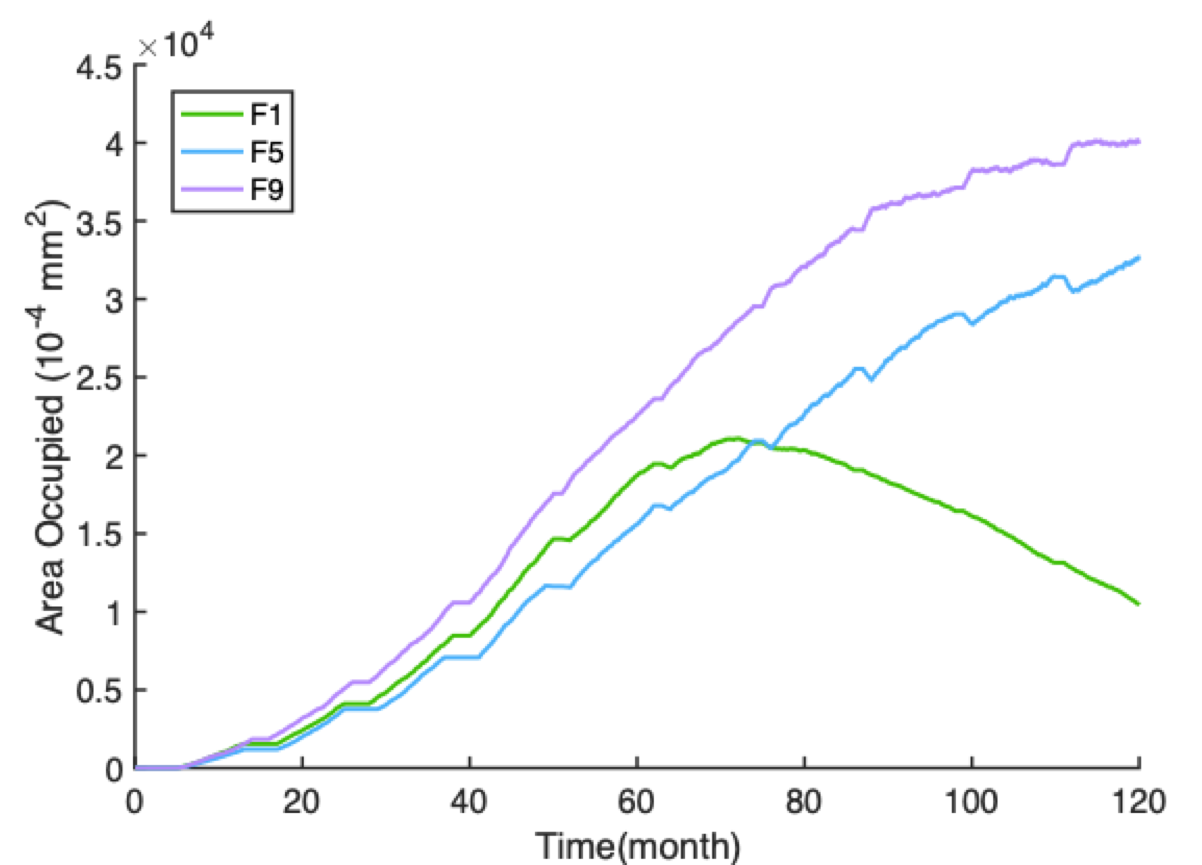
\includegraphics[height=4.2cm]{./formal/tropical/159[3].png}
	\caption{F1,F5,F9.}
	\label{pair1}
\end{minipage}   
\begin{minipage}{30.5ex}
\centering
	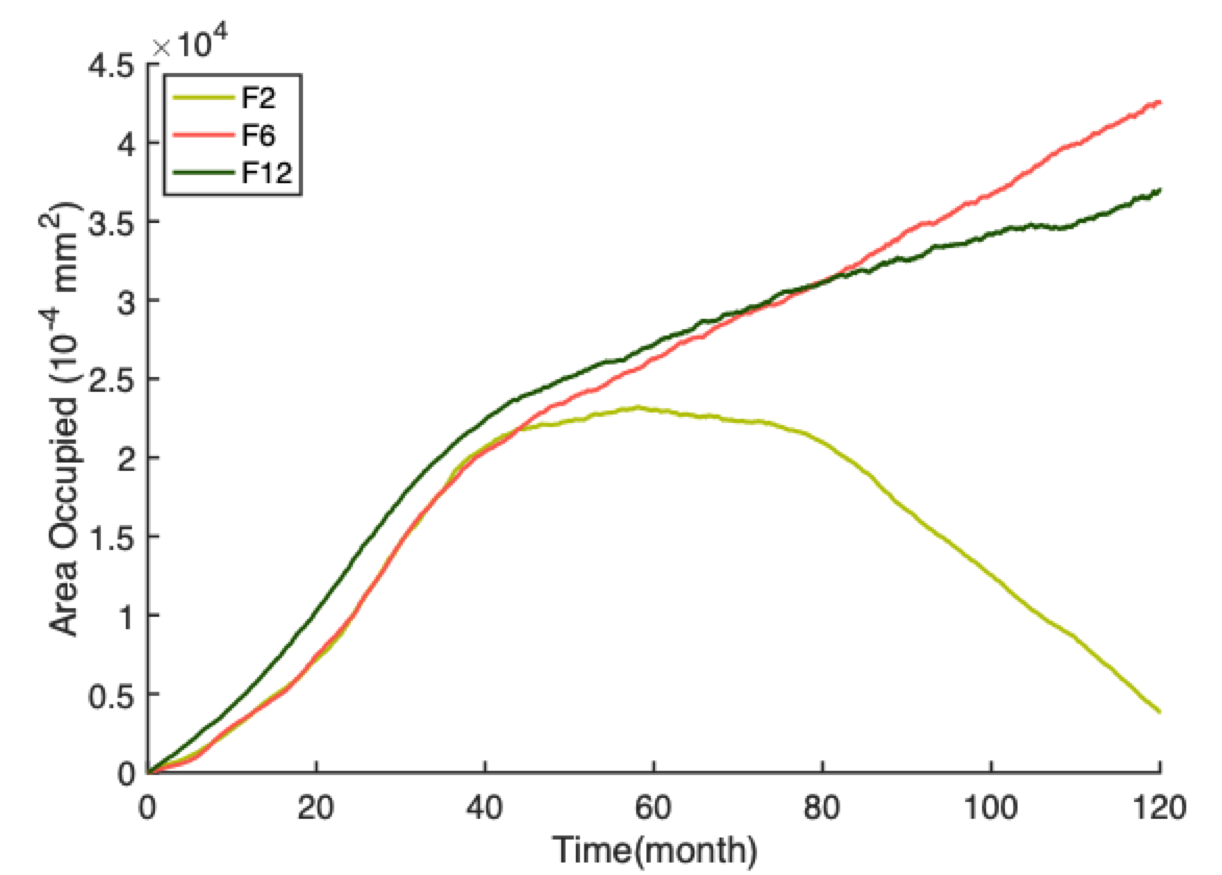
\includegraphics[height=4.2cm]{./formal/tropical/2612[2].png}
	\caption{F2,F6,F12.}
	\label{pair2}
\end{minipage}
\begin{minipage}{29ex}
\centering
	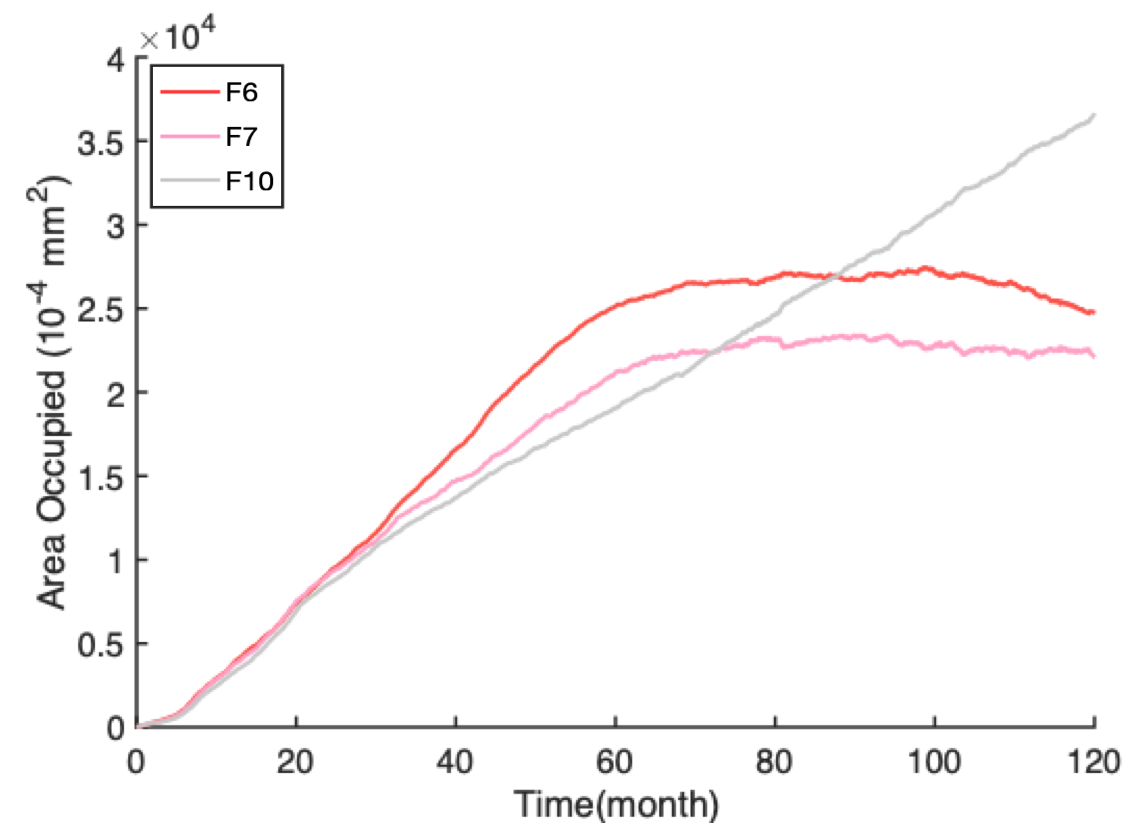
\includegraphics[height=4.2cm]{./formal/tropical/6710[3].png}
	\caption{F6,F7,F10.}
	\label{pair3}
\end{minipage} 
\end{figure}
Finally, we test the condition of all 11 fungi (except F8) and conclude that \textbf{F7 \& F10 }achieves the best, with \textbf{F4, F6, F9, F11, F12} following and can still live and grow for a certain amount (although being restrained). The result can also be obtained from Fig. \ref{t12} to Fig. \ref{yt12}.
\begin{figure}[]
\captionsetup{font={small}}
	\begin{minipage}{29ex}
	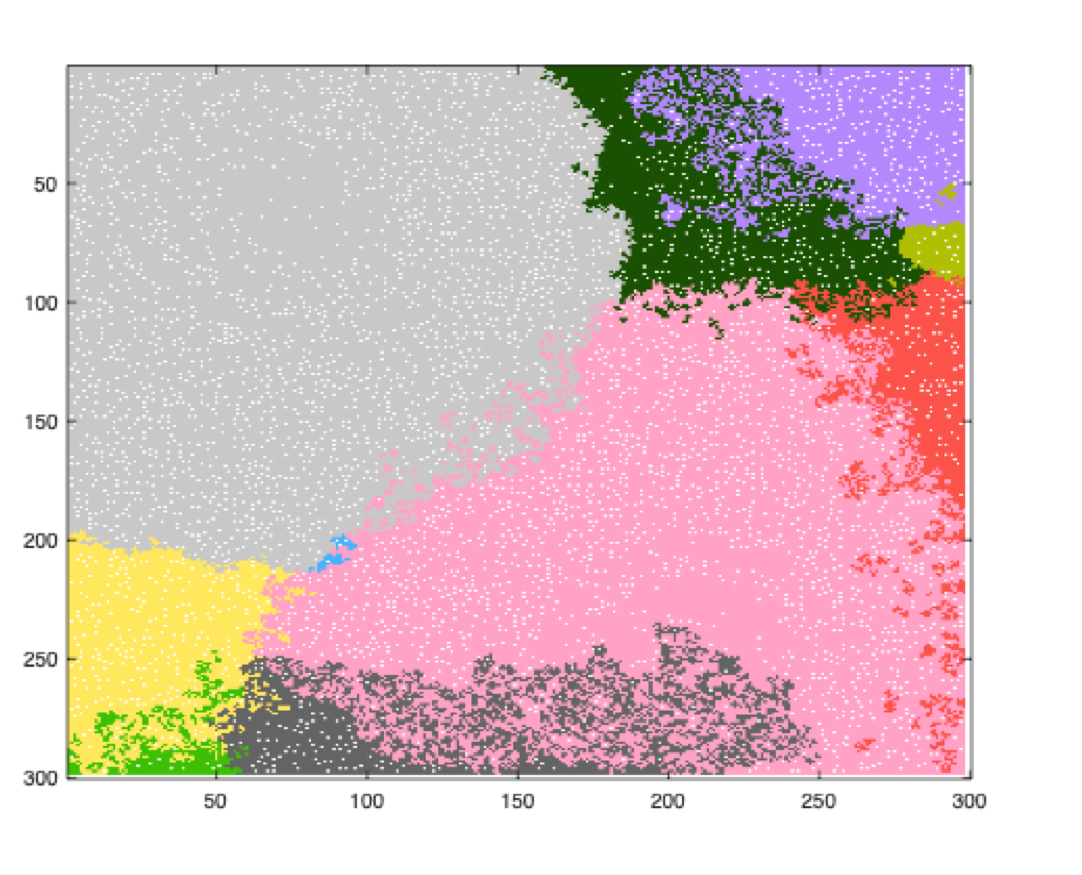
\includegraphics[height=4.8cm]{./formal/tropical/11[3].png}
	\caption{Ending condition.}
	\label{t12}
\end{minipage}   
\begin{minipage}{31ex}

	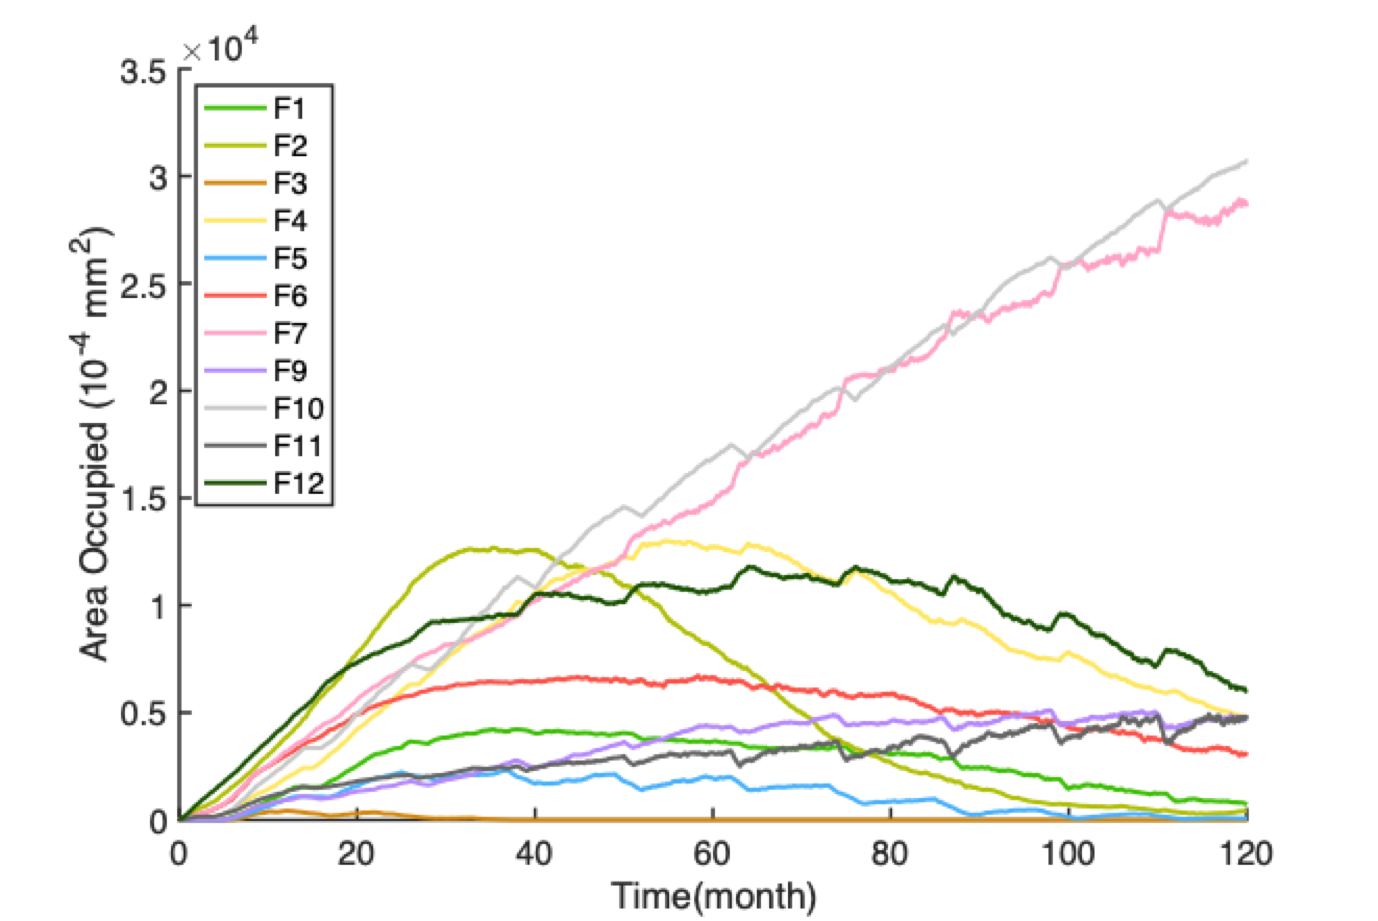
\includegraphics[height=4.3cm]{./formal/tropical/11[2].png}
	\caption{Curves in 10 years.}
\end{minipage}
\begin{minipage}{29ex}
\centering
	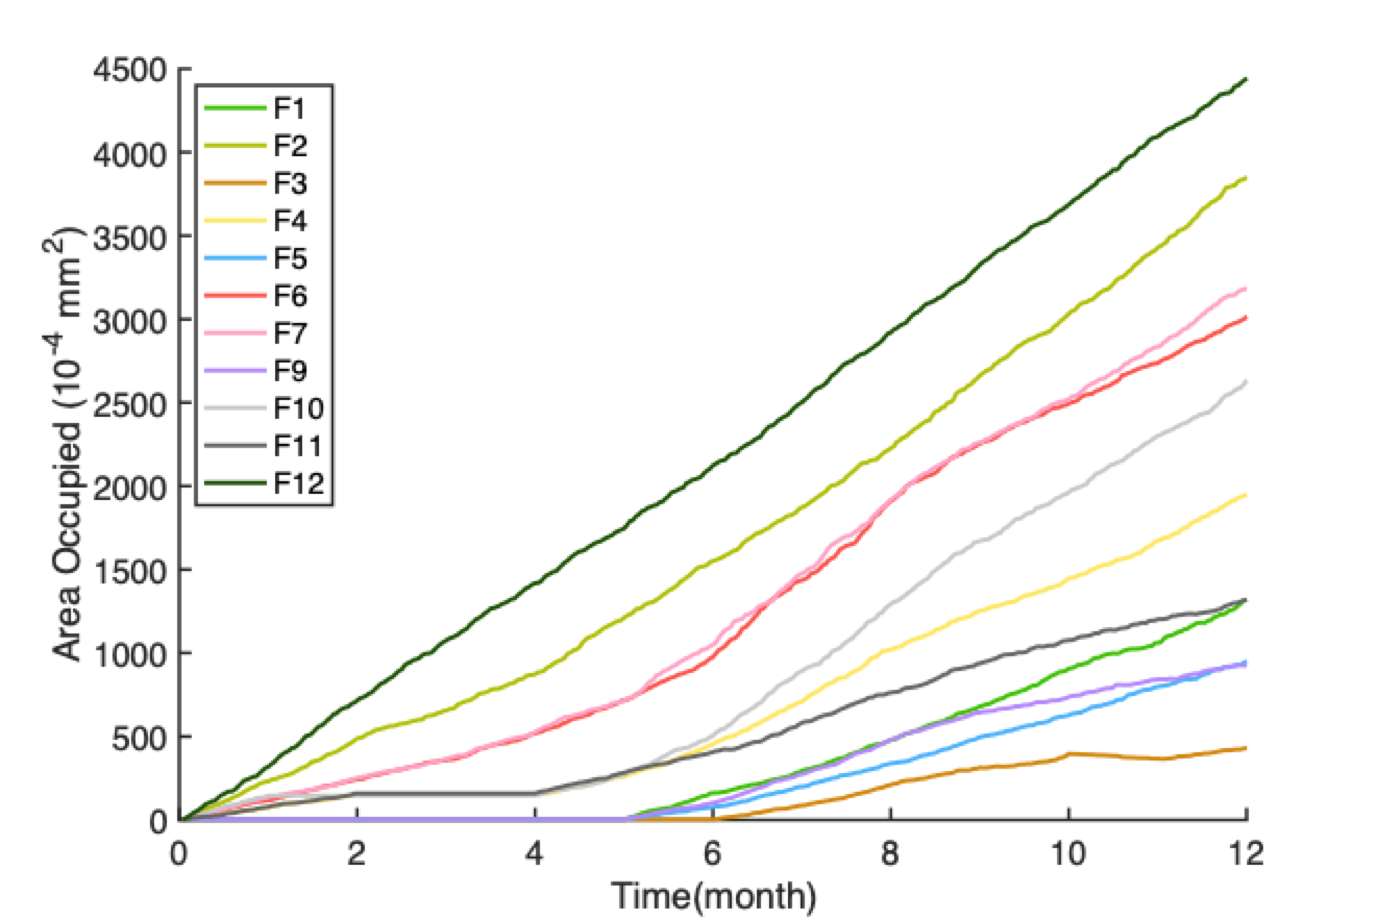
\includegraphics[height=4.2cm]{./formal/tropical/11[1].png}
	\caption{Yearly change.}
	\label{yt12}
\end{minipage} 
\end{figure}
Thus, the conclusion for the combinations under tropical rain forest is:
\begin{enumerate}
\setlength{\itemsep}{0ex} %条目间距
\item \textbf{Possible pairs: F5 \& F9, F6 \& F12, F6 \& F7}
\item \textbf{Possible groups: F4, F6, F9, F11, F12 and F4, F6, F7, F9, F10, F11, F12}
\end{enumerate} One thing to mention is that: \textbf{pairs selected from one group may not be able to persist well}, since the groups form a certain balance between species to ensure their persistence.


\newpage
\subsection{Arid climate}
Arid climate is famous for annually high temperature and low precipitation, thus create a great challenge for fungi growth. The list below summarized all the properties of 12 fungi under arid climate which is concluded from their annual growth behavior (which can also be partially reflected in Fig. \ref{a}).

\begin{enumerate}
\setlength{\itemsep}{0ex} %条目间距
\item \textbf{F4, F6, F7, F8, F10, F11:  Partially affected of around 7 month}\\
During roughly month 5-10, their growth is reduced due to high temperature and almost no precipitation. During month 1, their growth is reduced due to low precipitation. For the other time, they can still grow normally, but overall their extension speed is much lower because of low precipitation. 
\item \textbf{F5: Most stable}\\
According to its curve, F5 is not so affected by the annual weather change, thus it's the relatively stable one. But due to the severe environment, its growth is still reduced to some extent.
\item \textbf{F2, F9, F12: Partially hold-up}\\
During month 4-9, they all experienced a stop in growth due to bad climate condition. Since they have relatively close extension rate, they may exist better with each other. However, they have much less competitiveness among other stronger fungi.
\item \textbf{F3: Minor hold-up of 3 month}\\
F3 experienced no growth during month 6-8 due to the high temperature as well as low precipitation.  Its growth in other time is partially reduced but it can still maintain normal living. 
\item \textbf{F1: Comeplete dead}\\
F1 itself is not a strong fungus. Under such bad condition, we can't observe any evident growth.
\end{enumerate}

The result of the testing for the condition with all 12 fungi is shown in Fig.\ref{a12} to Fig. \ref{ya12}. We conclude that \textbf{F7 \& F10 }achieves the best, with \textbf{F4, F6, F9, F11, F12} following and can still live and grow for a certain amount (although being restrained).
\begin{figure}[]
\captionsetup{font={small}}
	\begin{minipage}{29ex}
	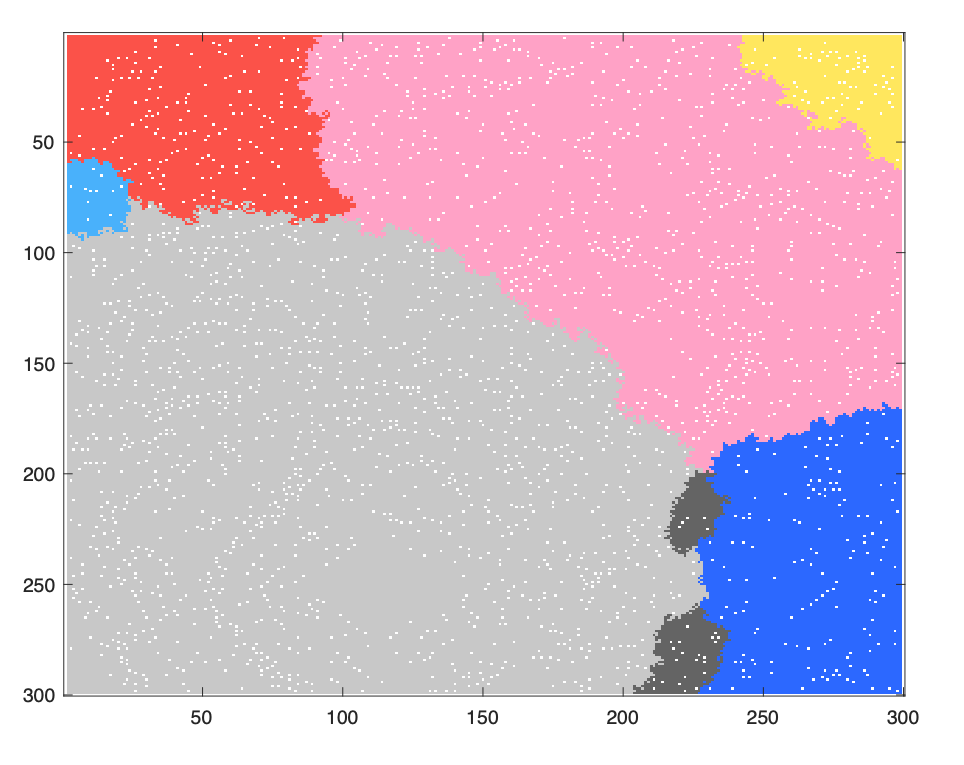
\includegraphics[height=4.2cm]{./formal/arid/12[3].png}
	\caption{Ending condition.}
	\label{a12}
\end{minipage}   
\begin{minipage}{31ex}
	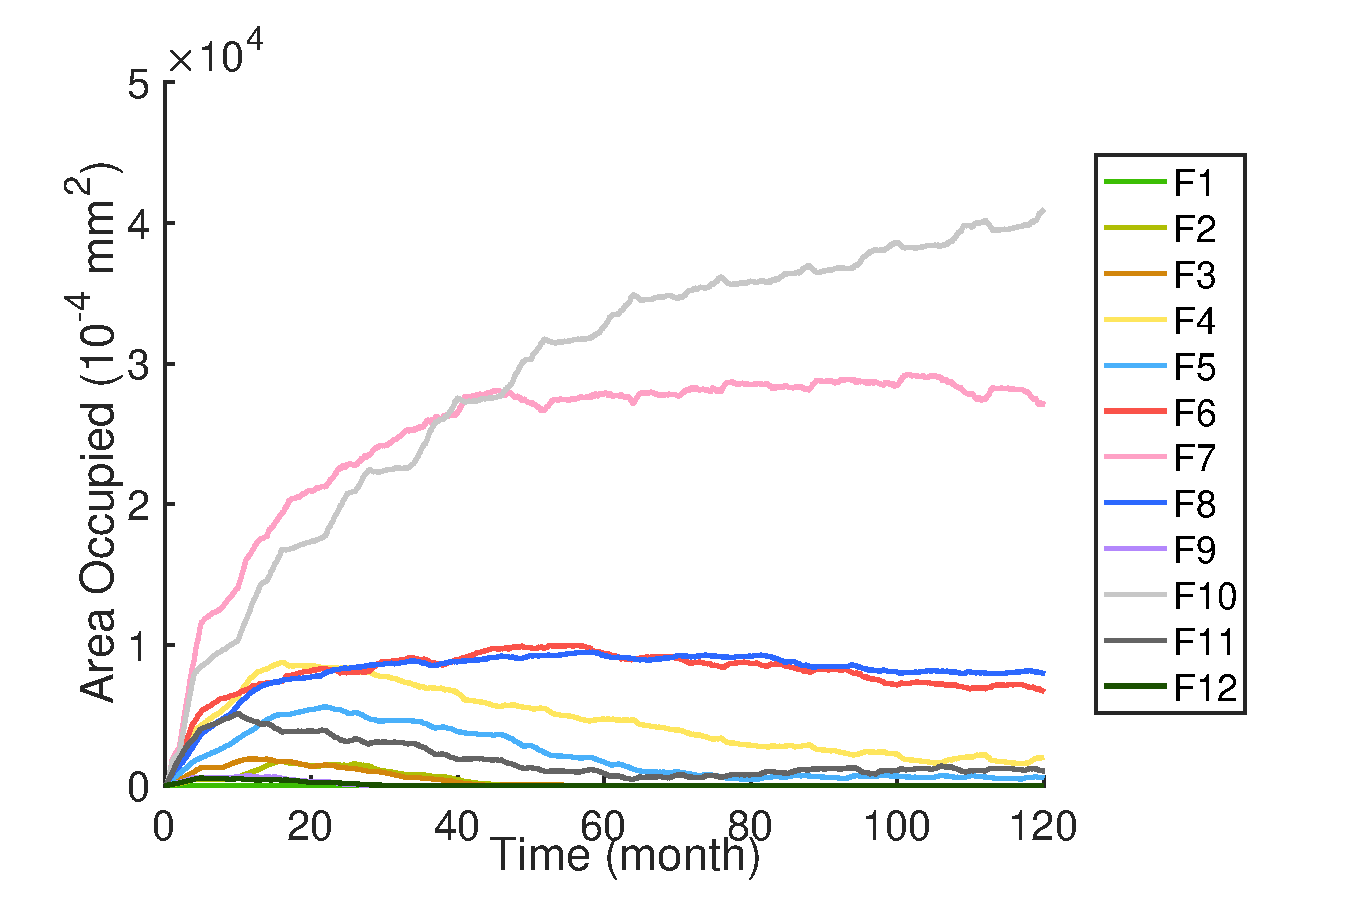
\includegraphics[height=4.2cm]{./formal/arid/12.eps}
	\caption{Curves in 10 years.}
	\label{a}
\end{minipage}
\begin{minipage}{29ex}
 \quad
	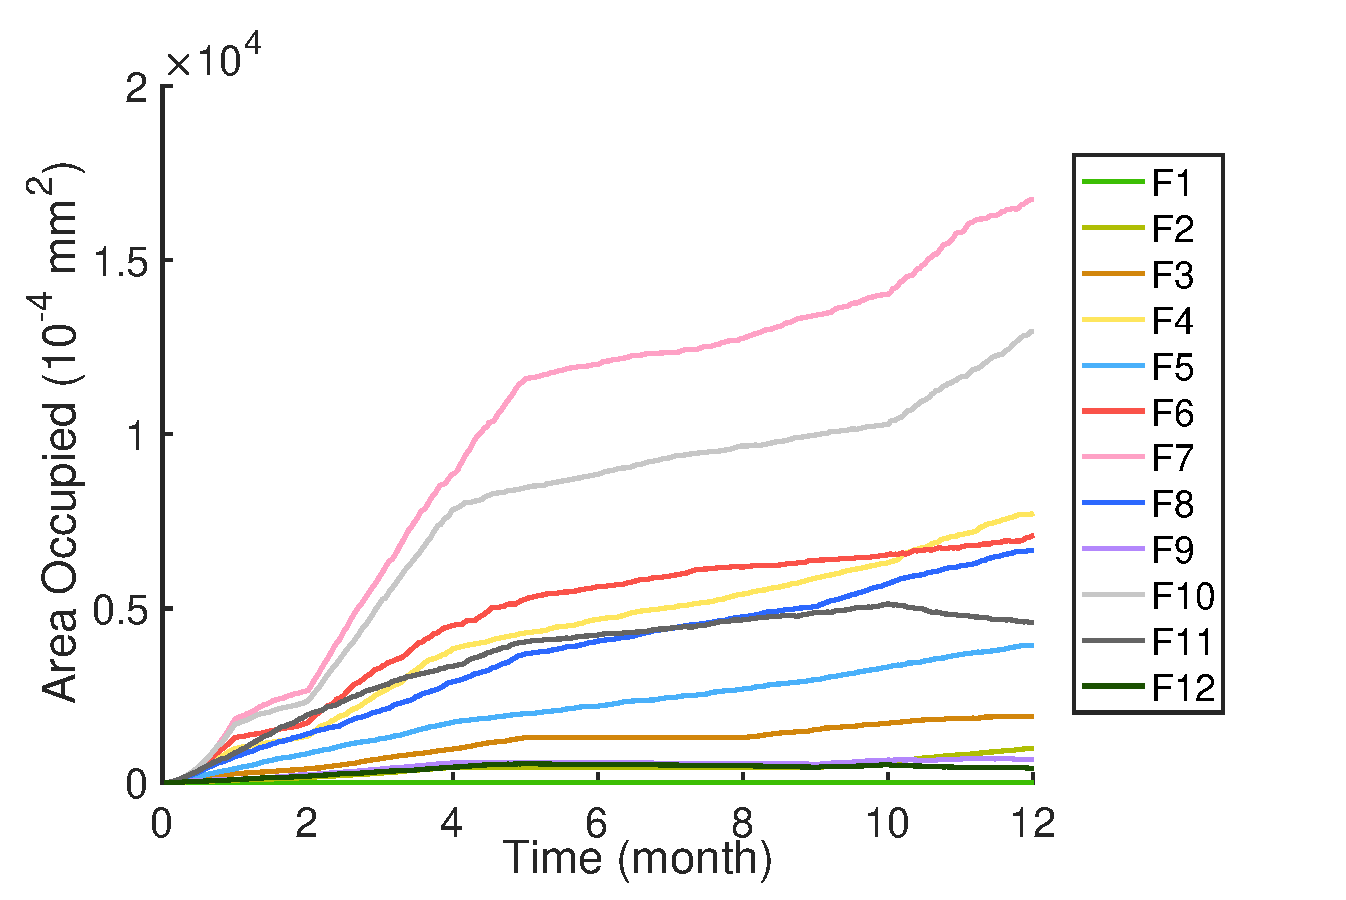
\includegraphics[height=4.2cm]{./formal/arid/12[2].eps}
	\caption{Yearly change.}
	\label{ya12}
\end{minipage} 
\end{figure}

Then, pairs and groups are found from the above division as well as the groups whose occupied area curve is closer to each other and tried one by one for testing. Below listed all the successful ones we found that can persist in a longer time period of ten years.
\begin{enumerate}
\setlength{\itemsep}{0ex} %条目间距
\item \textbf{Pairs:  F4 \& F7, F8 \& F10, F2 \& F3, F8 \& F11, F9 \& F12}
\item \textbf{Groups: F4, F5, F12 and F4, F6, F7, F8, F10}
\end{enumerate}


\subsection{Semi-arid}
Semi-arid is also a tough climate, although slightly better than arid. It has a normal temperature curve but still lack of precipitation (<50 mm). However, the fungi seems to be adapt most to such kind of environment. which can be seen from the advantage below that 8 can be categorized into stable. The conclusion of the advantage and disadvantage of all 12 fungi are listed below.
\begin{enumerate}
\setlength{\itemsep}{0ex} %条目间距
\item \textbf{F1, F2, F3, F4, F5, F9, F11, F12: Most stable} \\
All the six species can grow well under semi-arid climate. The effect of environmental change on their annual growth is not obvious and they can easily achieve a stable growth.
\item \textbf{F6, F7, F8, F10: Partially affected for 5 month}\\
During month 3-9 when temperature is relatively higher and there's some precipitation every day, the four species can achieve fastest growth. While in the other 5 month, their growth is reduced. Overall, they can still achieve a good extension thanks to their relatively higher extension rate.
\end{enumerate}

The result of the condition with all 12 fungi is shown in Fig.\ref{s12} to Fig. \ref{ys12} and we conclude that \textbf{F7 \& F8 \& F10 }achieves the best, with \textbf{F1, F4, F5, F6, F9, F11} following and can still grow for a certain amount (although being restrained).
\begin{figure}[H]
\captionsetup{font={small}}
	\begin{minipage}{29ex}
	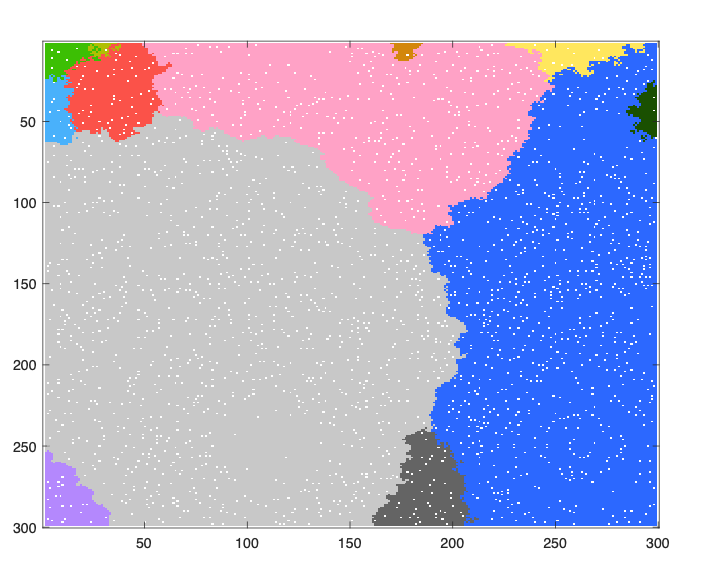
\includegraphics[height=4.4cm]{./formal/semi-arid/12[1].png}
	\caption{Ending condition.}
	\label{s12}
\end{minipage}   
\begin{minipage}{31ex}
	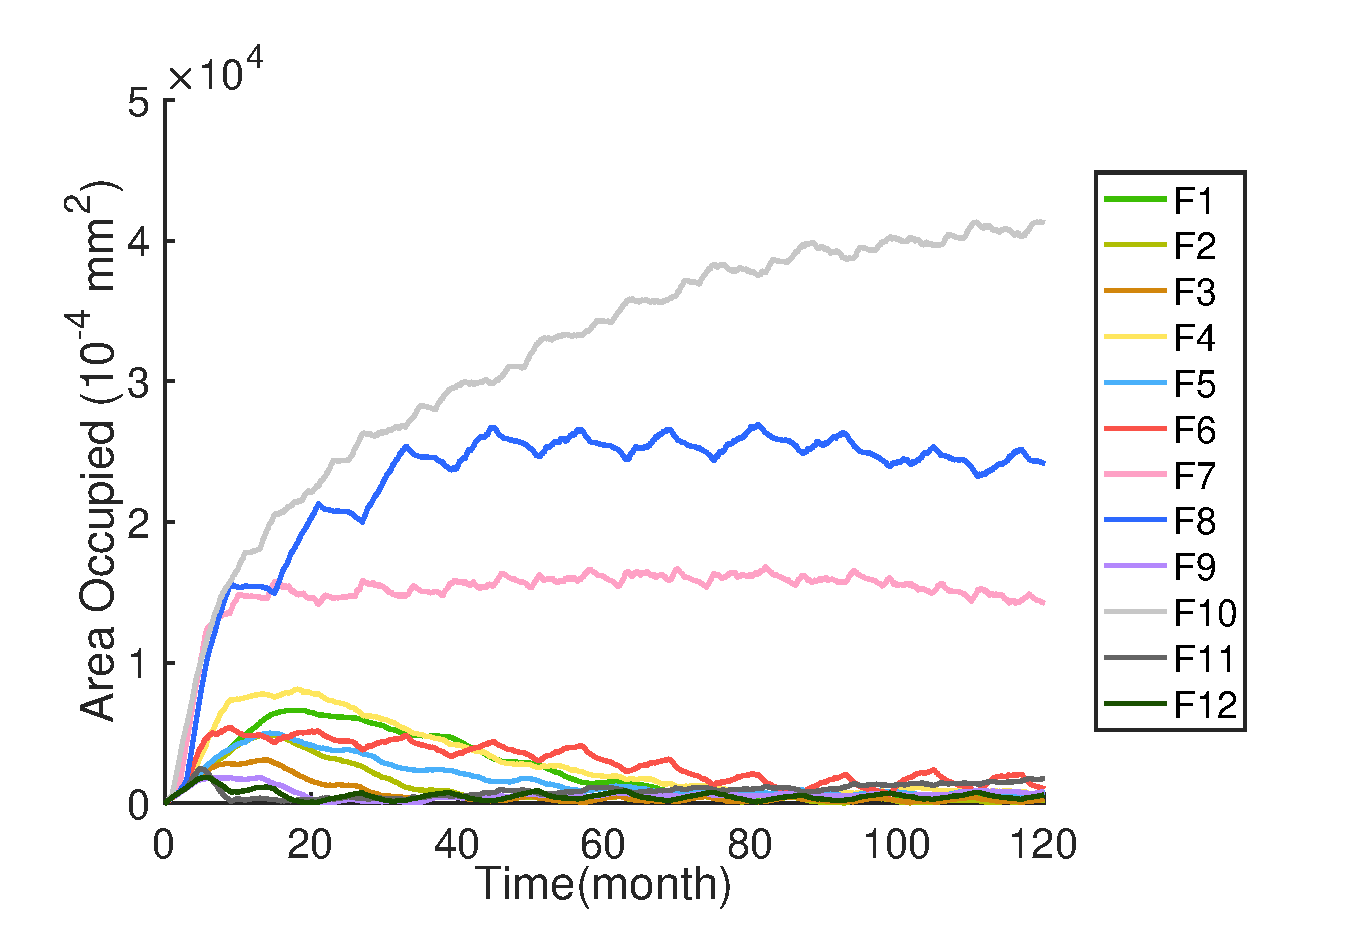
\includegraphics[height=4.3cm]{./formal/semi-arid/12[2].eps}
	\caption{Curves in 10 years.}
	\label{s}
\end{minipage}
\begin{minipage}{29ex}
 \quad
	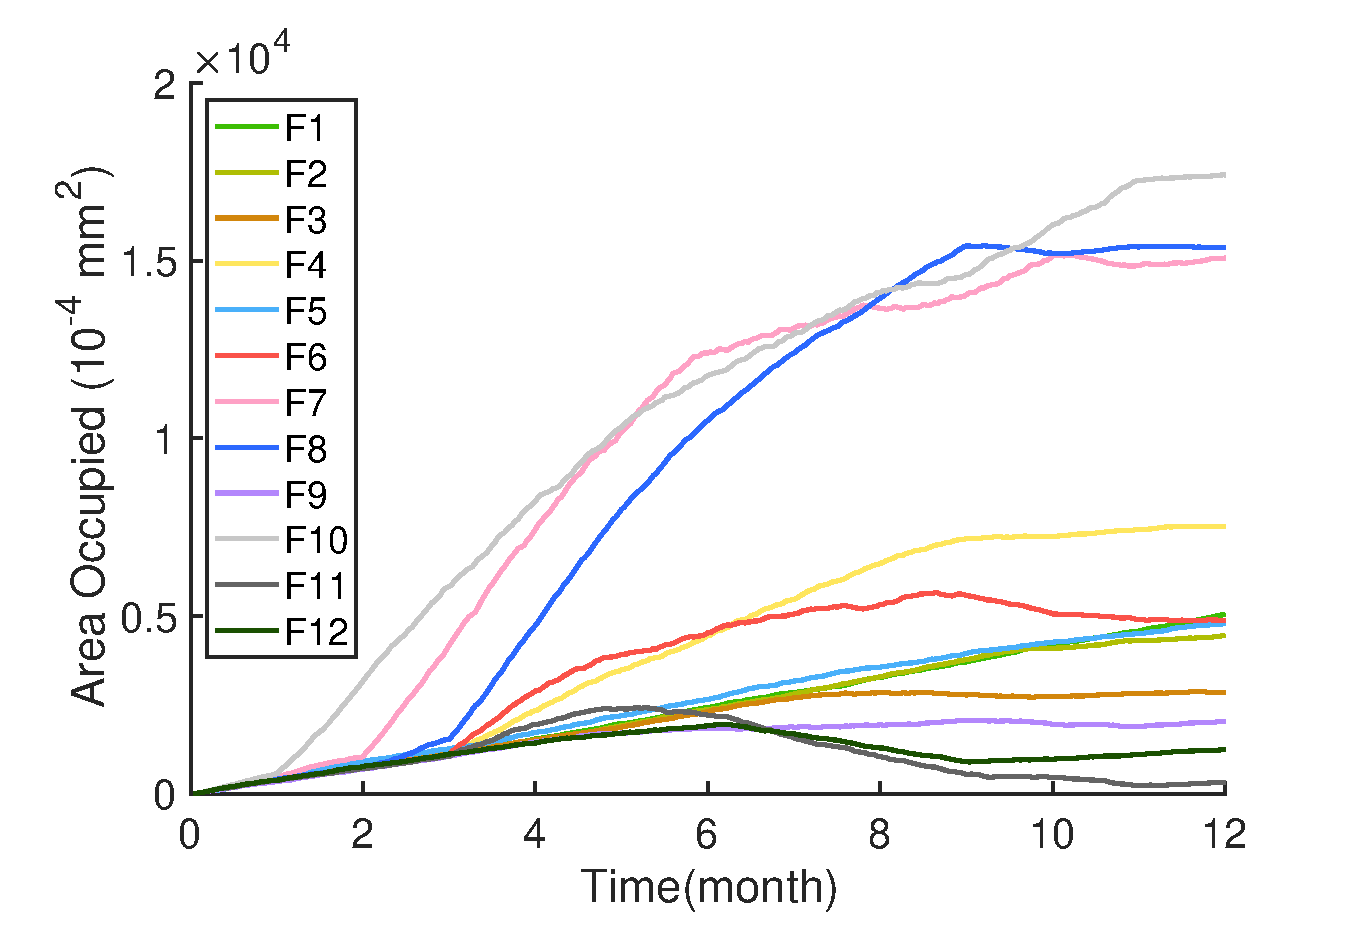
\includegraphics[height=4.2cm]{./formal/semi-arid/12[3].eps}
	\caption{Yearly change.}
	\label{ys12}
\end{minipage} 
\end{figure}

After enough testing, we've found some combinations that can persist under semi-arid, that is: 
\begin{enumerate}
\setlength{\itemsep}{0ex} %条目间距
\item \textbf{Pairs: F7 \& F8, F4 \& F6}
\item \textbf{Groups: F4, F5, F6, F9 and F5, F9, F12 and F7 \& F8 \& F10}
\end{enumerate}



\subsection{Temperate}
Temeperate weather is the coldest one among the five we've chosen with the warmest month less than 25 degrees and a medium precipitation of 50-100 mm. The city Boston we've tested in previous section is also included in this type of environment. 
\begin{enumerate}
\setlength{\itemsep}{0ex} %条目间距
\item \textbf{F1, F2, F3, F5, F9, F11, F12: Most stable} \\
Temperate is also a good climate condition for these fungi, since their annual growth is stable and through the area they've occupied we can conclude that their extension rate is also not largely affected. This means the weather lies mostly in their niche width for temperature and moisture.
\item \textbf{F4, F10: Largely affected} \\
There's only 2 month (7-8) when the growth of the two species is not reduced due to the relatively lower temperature that is not nice for F4 and 10. In other time period, their growth rate is sharply reduced which then makes them less competitive.
\item \textbf{F6: Minor affected for 2 month}\\
The condition for F6 is just the opposite as the previous set due to its temperature niche width. Thus F6 can achieve much better annual growth under such condition and easily catch up.
\item \textbf{F8: Partially affected for 4 month}\\
During winter, the growth of F7 decrease because of the low temperature. However, due to its high extension rate, such negative effect is not so dangerous for it to live on.
\item \textbf{F8: Fluctuation} \\
F8 is the only interesting phenomenon that is observed. During summer time, its growth may experience a clear fluctuation. Its growth rate may be reduced every month after another. This somehow slow down its annual average growth. But it can still make up by its relatively high extension rate.

\end{enumerate}

The result of the condition with all 12 fungi is shown in Fig.\ref{t12} to Fig. \ref{yt12} and we conclude that \textbf{F8}achieves the best, with \textbf{F8, F10} following and then \textbf{F1, F4, F5, F6, F9, F11} that can still grow for a certain amount (although being restrained).
\begin{figure}[H]
\captionsetup{font={small}}
	\begin{minipage}{29ex}
	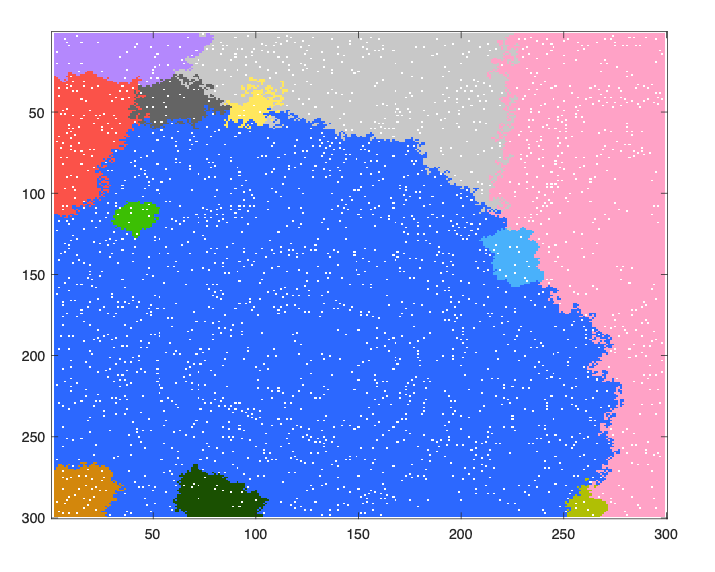
\includegraphics[height=4.4cm]{./formal/temperate/12[1].png}
	\caption{Ending condition.}
	\label{t12}
\end{minipage}   
\begin{minipage}{31ex}
	\includegraphics[height=4.4cm]{./formal/temperate/12[2].eps}
	\caption{Curves in 10 years.}
	\label{t}
\end{minipage}
\begin{minipage}{29ex}
 \quad
	\includegraphics[height=4.4cm]{./formal/temperate/12[3].eps}
	\caption{Yearly change.}
	\label{yt12}
\end{minipage} 
\end{figure}

Possible combinations for temperate climates includes:
\begin{enumerate}
\setlength{\itemsep}{0ex} %条目间距
\item \textbf{Pairs: F5 \& F9, F6 \& F7, F6 \& F11, F7 \& F8}
\item \textbf{Groups: F5, F6, F9, F11 }
\end{enumerate} Compare with parts of the result obtained in previous parts, we can see that the pair "F5 \& F9" appears again, which shows some degree of reliability of our model.


\subsection{Arboreal}
Arboreal is a relatively nicer climate for human as well as for fungi with 6 species being stable enough to external weather fluctuations. Luckily, it's also the second climate which is suitable for fungus F8 and it can eat up any other species along with it. Thus, from now on in this subsection, we \textbf{remove F8 temporarily} when testing.
\begin{enumerate}
\setlength{\itemsep}{0ex} %条目间距
\item F1, F2, F3, F5, F9, F12:  Most stable \\
With no danger around, their growth curves are highly slmilar and stable all year round. Comparing the area occupied, we can also see a slight increase which means arboreal is better for them to live.
\item F4, F7, F10: Largely affected \\
For these three species, they only grow at fastest condition during month 9-10. In other time period, they growth rate is sharply declined.
\item F8: Minor affected for around 3 month\\
During winter F8 is afffected by the low temperature which limits its growth. But in the other time since F8 has a high extension rate, it can soon catch up.
\item F6: Partially affected for 6 month \\
In summer due to the slightly higher temperature, the growth rate of F6 is reduced. It's a disadvantage for it when other fungi are possibly at their best conditon.

\end{enumerate}


The result of the condition with all 12 fungi is shown in Fig.\ref{ar12} to Fig. \ref{yar12} and we conclude that \textbf{F9, F10, F11}achieves the best, with \textbf{F1, F2, F4, F5, F6, F12} that can still grow for a certain amount (although being restrained).
\begin{figure}[H]
\captionsetup{font={small}}
	\begin{minipage}{29ex}
	\includegraphics[height=4.4cm]{./formal/arboreal/12[1].png}
	\caption{Ending condition.}
	\label{ar12}
\end{minipage}   
\begin{minipage}{31ex}
	\includegraphics[height=4.3cm]{./formal/arboreal/12[2].eps}
	\caption{Curves in 10 years.}
	\label{ar}
\end{minipage}
\begin{minipage}{29ex}
 \quad
	\includegraphics[height=4.2cm]{./formal/arboreal/12[3].eps}
	\caption{Yearly change.}
	\label{yar12}
\end{minipage} 
\end{figure}


For the final environment arboreal, the possible "partners" are listed as follows:
\begin{enumerate}
\setlength{\itemsep}{0ex} %条目间距
\item \textbf{Pairs: F1 \& F4 }
\item \textbf{Groups: F9, F10, F11 and F1, F4, F5, F6, F9}
\end{enumerate}


\section{Importance of Biodiversity}

\par As introduced in Section 1, the breakdown of ground litter is an important process in ecological cycles. Therefore, the efficiency of decomposition is one of the determinants of the efficiency of ecosystems. In order to study the importance of species diversity of fungi, we are going to test whether the diversity of species will improve the efficiency of decomposition and adaptation to variable environments.
\subsection{Fungi Combination Selection}
\par First of all, according to the results of the previous models, we can get the following rules on the selection of fungi.
\begin{itemize}
\setlength{\itemsep}{0ex} %条目间距
	\item According to the analysis of XXXXXX(task 1 name) and xxxxx(task Boston name), we need to choose species that can coexist peacefully on long-term trends to ensure the \textbf{stability of biodiversity}.
	\item From xxxxx(fluctuation model name), we can know that the decomposition rate of fungus is sensitive to environmental changes, so the \textbf{adaptability and viability} of fungi are considered prior to the expansion rate of fungi. Moreover, when different fungi are combined, the temperature and moisture niche width that the whole system have should be maximized.
	\item When the above two conditions are satisfied as much as possible, we should choose the combination of fungi that expand as fast as possible, because they show great advantages when we do not consider the environmental impact in our initial model.	
\end{itemize}
\par So that according to the previous rules, we can set 5 groups with the same initial numbers of fungi and the same initial positions. 
\vspace{-0.3cm}
\begin{table}[H]
	\centering
	\caption{Groups Setting}
	\begin{tabular}{|c|c|c|c|c|c|}
		\hline
		&Group 1 & Group 2 & Group 3 & Group4& Group5\\
		\hline 
		Fungi choose&F3 $\times$ 4 & F9 $\times$ 4 & F3 $\times$ 2 \& F5 $\times$ 2 &  F11 $\times$ 2 \& F12 $\times$ 2 & F7, F8, F11, F12\\
		\hline
		Moisture width &1.32&1.57&1.35&5.17&5.17 \\
		\hline
		Temperature width &15.8&18.6&25.0&28.5&29.1 \\
		\hline
	\end{tabular}
\end{table}

\subsection{Results}
\par In the simulation of this section, we fixed the trend of temperature and moisture to be similar to that of semi-arid area and use cellular automata model to run for 1000 days. The following Fig.\eqref{SYHD} shows theremaining wood thickness for the five different groups of fungi.
\begin{figure}[H]
	\centering
	\begin{subfigure}{0.3\textwidth}
		\includegraphics[width=\textwidth]{./T5Figure/K1N1/K1N1L.pdf}
		\caption{F3}
	\end{subfigure}
	\begin{subfigure}{0.3\textwidth}
		\includegraphics[width=\textwidth]{./T5Figure/K1N2/K1N2L.pdf}
		\caption{F9}
	\end{subfigure}
	\begin{subfigure}{0.3\textwidth}
		\includegraphics[width=\textwidth]{./T5Figure/K2N1/K2N1L.pdf}
		\caption{F3 F5}
	\end{subfigure}
	\begin{subfigure}{0.3\textwidth}
		\includegraphics[width=\textwidth]{./T5Figure/K2N2/K2N2L.pdf}
		\caption{F11 F12}
	\end{subfigure}
	\begin{subfigure}{0.3\textwidth}
		\includegraphics[width=\textwidth]{./T5Figure/K4N1/K4N1L.pdf}
		\caption{F7 F8 F11 F12}
	\end{subfigure}
	\caption{Remaining wood thickness.}
	\label{SYHD}
\end{figure}

\par In order to analyze the process better, we draw the change relationship of the remaining proportion of trees during the process. We set the overall thickness of the wood very large in order to maintain the stability of the system.
\vspace{-0.5cm}
\begin{figure}[H] 
	\centering 
	\includegraphics[height=6.2cm]{./T5Figure/T5overAll.eps}
	\caption{Changes in mass of wood.}
	\label{BHQX}
\end{figure}
\vspace{-0.3cm}
\par From Fig.\eqref{BHQX}, we can conclude that when environmental factors are taken into account, biodiversity affects the decomposition rate of fungi. When the total number of fungi and the changing trend of the environment remained unchanged, the decomposition efficiency of the system with four different kind of fungi can reach \textbf{twice} as high as that of a single kind and \textbf{1.25 times} as high as that of two kinds.
\par However, there are preconditions for the conclusion in the previous paragraph, which are \textbf{stability of biodiversity} and \textbf{adaptability and viability} of fungi. Only when these conditions are fully met can we say that the system has \textbf{real biodiversity}


\section{Conclusion}
In this whole project,we're discussing the importance of the role fungi play in carbon cycle: decomposing wood material and litters. Factors include environmental fluctuation, competition between species, overall climate condition as well as the diversity of species are considered to explore their effect on fungi's growth and wood decomposition.

First, we use mathematic modeling to simulate the whole decomposition process. The decomposition rate is calculated accurately considering only two main factors: extension rate and moisture tolerance. The compete rankings are set using Elo system. And finally CA modeling is used to show the process of competition and dynamic growth of the fungi. To make the result more vivid, we add visualization such as mapping, line charts and surface plot.

Then we add the environmental fluctuation and variation of weather patterns into our model to further modify the extension and decomposition rate of each fungus, considering their best growing temperature and moisture range. We categorized 2v2 competition into different endings. By comparing the competition result and the curves they present before and after adding external environment change, we conclude that environmental change not only affect their normal growth, making their curve less smooth, but also increase the time stronger fungus needs to win with the possibility of even reversing the win-lose  situation.

After that, we increase the competition into 12 species and five different climates: tropical, arid, semi-arid, temperate and arboreal. For each climate, we categorized all 12 fungi into different advantages and disadvantages regarding the annual weather change. Also, we predict the possible combination of fungi species again using the established model.

Finally, we considered the influence diversity has on the decomposition of wood materials. By comparing different species with the same total number growing in same condition and their consumption of the wood, we conclude that a rich biodiversity has an obvious positive effect on the efficiency of consuming materials, thus pushing the whole carbon cycling system.

\section{Sensitivity Analysis}
\par In section 5.4, we have proved that our model is \textbf{sensitive to the rapid and drastic changes of temperature and moisture}. This is because different fungi have different optimal temperature and moisture. In our model, although the behavior pattern of each cell is complex, the overall behavior pattern of fungi is predictable according to some existing rules and our simulation results is exactlky consistent with these rules.
\par \textbf{Initial location} is also an important factor affecting the final results. So in the process of solving all the previous models, the initial position of fungi is fixed. Here we tested whether the initial position of fungi will have a great impact on the final area occupied by it when there are multiple fungi exists.
\par The following Fig.\eqref{qwert} shows the results of the sensitivity analysis of the initial position. We fix the temperature and moisture and choose three different fungi (F5/F9/F12) for testing. Before each run of the cellular automata, we randomly generate initial positions for the three fungi and repeate the simulation for 50 times. Finally, we fit three curves for them using Matlab and because the slope of the three curves is close to 0, we can conclude that our model is \textbf{insensitive to the initial position of the fungus when the number of tests is large enough}.
\vspace{-0.3cm}
\begin{figure}[H] 
	\centering 
	\includegraphics[height=6cm]{./picture/sensitivity.pdf}
	\caption{Algorithm schematic}
	\label{qwert}
\end{figure}

\section{Strength and Weakness}
\subsection{Strength}
\begin{itemize}
\setlength{\itemsep}{0ex} %条目间距
	\item A scientific and accurate simulation model is established by using \textbf{cellular automata} in MATLAB. \textbf{Excellent visualization} of fungal growth process makes the output of the model more intuitive, and also adds a lot of fun when solving the model.
	\item \textbf{Continuous problem discretization}: It is easy to update the model and consider more influence factors. It also enhances the robustness of the model and makes the model more stable.
	\item We simulate the change and influence of temperature and moisture in a very \textbf{large range}, including long-term and short-term simulation under eight different conditions (Boston/completely random environment/fixed value/five climate types).
\end{itemize} 
\subsection{Possible Improvements}
\begin{itemize}
\setlength{\itemsep}{0ex} %条目间距
	\item In our model, we only consider the competition relationship between fungi, but there are \textbf{other relationships} between them, such as cooperation.
	\item As the model becomes larger and larger, the \textbf{time} required to run a simulation code will become correspondingly longer. So when all the factors were taken into account, the computer is not fast enough to support the interaction of more than ten fungi on too many cells.
\end{itemize}


\begin{thebibliography}{20}
\setlength{\itemsep}{-0.5mm}
		\bibitem{CompArticle}
		Lustenhouwer, Nicky et al "A trait-based understanding of wood decomposition by fungi." Proceedings of the National Academy of Sciences 117.21 (2020): 11551-11558. Web. 05 Feb. 2021.
		\bibitem{mushroom}
        "fungi". URL: https://image.baidu.com/search/detail?ct=503316480\&z=0\&ipn=d\&word
 		 \bibitem{Nature}
        Maynard, D.S., Bradford, M.A., Covey, K.R. et al. "Consistent trade-offs in fungal trait expression across broad spatial scales". Nat Microbiol 4, 846–853 (2019). URL: https://doi.org/10.1038/s41564-019-0361-5
		
		\bibitem{MCM}
		"Problem A"
		\bibitem{chess}
		 A. E. Elo, The Rating of Chessplayers, Past and Present (Arco, 1978).
		 
        \bibitem{weather}
        National Weather Service Forecast Office. "Boston, Ma; Monthly Weather Summary (CLM)". URL: https://w2.weather.gov/climate/index.php?wfo=box


		\bibitem{climate}
Arnfield, A. John. "Köppen climate classification". Encyclopedia Britannica, 11 Nov. 2020, https://www.britannica.com/science/Koppen-climate-classification. Accessed 6 February 2021.
		\bibitem{climate2}
		"Climate Classification and Climatic Regions of the World". Fundamentals Of Physical Geography, 2nd Ed. Chapter 7. web:physicalgeography.net. URL:http://www.physicalgeography.net/fundamentals/7v.html
		\bibitem{arboreal}
		Elizabeth Murigi. "What Are The Characteristics Of An Oceanic Type Of Climate?". web:worldatlas.com. Feb 5, 2018. URL:https://www.worldatlas.com/articles/what-are-the-characteristics-of-an-oceanic-type-of-climate.html
		\bibitem{ocean}
		Gravity Wiki."Oceanic climate". web. URL: https://gravity.wikia.org/wiki/Oceanic\_climate
		\bibitem{mois-pre}
        "Fitting formula and empirical formula of mean precipitation and relative humidity". 2016. URL: http://blog.sciencenet.cn/blog-1458267-991122.html

		\end{thebibliography}
		
		
		
\begin{appendix}


\section{Fungus species data}

\begin{table}[H]
                \centering
                \caption{Fungi data}
                \begin{tabular}{|c|c|c|c|c|c|c|c|}
                \hline
                    & Name                                    & $E_0$ & $T_{min}$ & $T_{max}$ & $m_{min}$ & $m_{max}$ & R     \\ \hline
                F1  & Armillaria\_gallica\_FP102531\_C6D      & 0.25  & 6.4       & 31.1      & 0.45      & 3.46      & 0.232 \\ \hline
                F2  & Armillaria\_gallica\_HHB12551\_C6C      & 0.49  & 15        & 31.2      & 0.19      & 4.34      & 0.000 \\ \hline
                F3  & Armillaria\_tabescens\_TJV93\_261\_A1E  & 1.07  & 16.3      & 32.1      & 0.11      & 1.43      & 0.000 \\ \hline
                F4  & Fomes\_fomentarius\_TJV93\_7\_A3E       & 4.71  & 20.8      & 30.1      & 0.1       & 1.29      & 0.285 \\ \hline
                F5  & Hyphodontia\_crustosa\_HHB13392\_B7B    & 1.96  & 7.1       & 30.3      & 0.09      & 1.28      & 0.569 \\ \hline
                F6  & Lentinus\_crinitus\_PR2058\_C1B         & 6.38  & 22.4      & 40.2      & 0.13      & 1.68      & 0.569 \\ \hline
                F7  & Merulius\_tremullosus\_FP102301\_C3E    & 10.62 & 16.6      & 34.2      & 0.12      & 1.31      & 0.788 \\ \hline
                F8  & Phlebiopsis\_flavidoalba\_FP150451\_A8G & 10.8  & 15.7      & 32.7      & 0.27      & 2.81      & 0.986 \\ \hline
                F9  & Phellinus\_hartigii\_DMR94\_44\_A10E    & 1.54  & 9.6       & 28.2      & 0.42      & 1.99      & 0.493 \\ \hline
                F10 & Phlebia\_acerina\_MR4280\_B9G           & 8.75  & 13.6      & 31.3      & 0.1       & 1.29      & 1.000 \\ \hline
                F11 & Tyromyces\_chioneus\_HHB11933\_B10F     & 3.88  & 19        & 33.6      & 0.08      & 1.27      & 0.805 \\ \hline
                F12 & Xylobolus\_subpileatus\_FP102567\_A11A  & 0.77  & 5.1       & 33.6      & 0.29      & 5.25      & 0.493 \\ \hline
                \end{tabular}
                \end{table}
                
\end{appendix}


\newpage 
\begin{figure}[H]
        \includepdf[width=\paperwidth]{article1.pdf}
\end{figure}
\newpage 
\begin{figure}[H]
    \includepdf[width=\paperwidth]{article2.pdf}
\end{figure}




\end{document}

